\part{Fundamental electromagnetic principles and magnetic materials}
\title[Electromagnetic and material fundamentals]{Fundamental electromagnetic principles and magnetic materials}  
\date{}  
\frame{\titlepage} 

%%%%%%%%%%%%%%%%%%%%%%%%%%%%%%%%%%%%%%%%%%%%%%%%%%%%%%%%%%%%%
%% Ampere's circuital law: magnetic field strength %%
%%%%%%%%%%%%%%%%%%%%%%%%%%%%%%%%%%%%%%%%%%%%%%%%%%%%%%%%%%%%%
\begin{frame}
	\frametitle{Amp\`ere's circuital law: magnetic field strength}
	\begin{columns}
		\begin{column}{0.55\textwidth}
			Relates the circulation of a magnetic field around a closed loop to the electric current passing through the loop:
            \begin{align}
                \mbox{Integral form:} \quad &\oint_{\partial S} \bm{H} \cdot \mathrm{d}\bm{s} = I_{\mathrm{f}},\\
                \mbox{Differential form:} \quad &\nabla \times \bm{H} = \bm{J}_{\mathrm{f}}. 
                \label{eq:ampere_law}
            \end{align}
            Here, $\bm{H}$ is the magnetic field strength, $\bm{J}_{\mathrm{f}}$ is the free current density, and $I_{\mathrm{f}}$ is the free current enclosed by the loop $\partial S$. 
            \vspace{0.25cm}
            \begin{itemize}
                \item<2-> Free current: current that is not bound to a material (i.e., without polarization and magnetization currents).
                \item<3-> SI-units: $[H] = \si{\ampere\per\metre}$, $[J] = \si{\ampere\per\metre\squared}$
            \end{itemize}
		\end{column}
        \hfill
		\begin{column}{0.4\textwidth}
			\begin{figure}
				\centering
				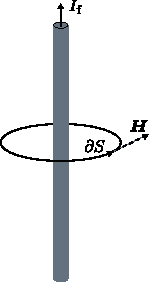
\includegraphics[height=0.7\textheight]{fig/lec02/Magnetic_field_strength_simple_conductor.pdf}
				\caption{Illustration of the magnetic field strength $\bm{H}$ around a simple conductor}
			\end{figure}
		\end{column}
		\end{columns}
\end{frame}

%%%%%%%%%%%%%%%%%%%%%%%%%%%%%%%%%%%%%%%%%%%%%%%%%%%%%%%%%%%%%
%% Ampere's circuital law: free current example %%
%%%%%%%%%%%%%%%%%%%%%%%%%%%%%%%%%%%%%%%%%%%%%%%%%%%%%%%%%%%%%
\begin{frame}
	\frametitle{Amp\`ere's circuital law: free current example}
	\begin{columns}
		\begin{column}{0.55\textwidth}
			What is the free current $I_{\mathrm{f}}$ enclosed by the loop $\partial S$?
            \begin{itemize}
                \item<2-> The current $I_1$ flows in the direction of the loop $\partial S$ (according to right-hand rule).
                \item<3-> The current $I_1$ must be counted $N$ times due to the $N$ turns of wire around the loop $\partial S$.
                \item<4-> The current $I_2$ flows in the opposite direction of the loop $\partial S$ (according to right-hand rule).
                \item<5-> Result:
            \end{itemize}
            \vspace{0.25cm}
            \onslide<5->{\begin{equation*}
                I_\mathrm{f} = N \cdot I_1 - I_2.
            \end{equation*}}
		\end{column}
        \hfill
		\begin{column}{0.45\textwidth}
			\begin{figure}
				\centering
				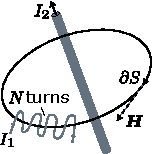
\includegraphics[height=0.5\textheight]{fig/lec02/Magnetic_field_strength_multiple_conductors.pdf}
				\caption{Arrangement with two electrical conductors}
			\end{figure}
		\end{column}
		\end{columns}
\end{frame}

%%%%%%%%%%%%%%%%%%%%%%%%%%%%%%%%%%%%%%%%%%%%%%%%%%%%%%%%%%%%%
%% Ampere's circuital law: simple solenoid  example%%
%%%%%%%%%%%%%%%%%%%%%%%%%%%%%%%%%%%%%%%%%%%%%%%%%%%%%%%%%%%%%
\begin{frame}
	\frametitle{Amp\`ere's circuital law: simple solenoid example}
	\begin{columns}
		\begin{column}{0.575\textwidth}
			Ampere's law for magnetic flux density $\bm{B}$ in vacuum:
            \begin{align}
                \mbox{Integral form:} \quad &\oint_{\partial S} \bm{B} \cdot \mathrm{d}\bm{s} = \mu_0 I,\\
                \mbox{Differential form:} \quad &\nabla \times \bm{B} = \mu_0\bm{J}. 
            \end{align}
            Here, $\mu_0$ is the permeability of free space, $\bm{J}$ is the total current density and $I$ is the total current enclosed by the loop $\partial S$. 
            \vspace{0.25cm}
            \begin{itemize}
                \item<2-> SI-unit: $[B] = \si{\tesla} = \si{\volt\second\per\metre\squared} = \si{\newton\per\ampere\per\metre}$
                \item<3-> Example contour $\partial S$  on the right covering $N$ turns and length $l$ (flux density within solenoid):
            \end{itemize}
            \onslide<4->{$$\oint_{\partial S} \bm{B} \cdot \mathrm{d}\bm{s} = N \mu_0 I  \Leftrightarrow B = \frac{N \mu_0 I}{l}$$}
		\end{column}
        \hfill
		\begin{column}{0.425\textwidth}
            \vspace{-0.2cm}
			\begin{figure}
				\centering
				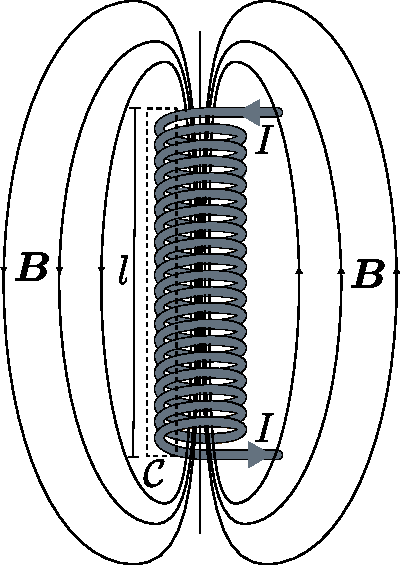
\includegraphics[height=0.68\textheight]{fig/lec02/Solenoid_Ampere_law.pdf}
				\caption{Magnetic flux $\Phi$ evaluated at the surface $\bm{S}$  (adapted from: \href{https://commons.wikimedia.org/wiki/File:Solenoid_and_Ampere_Law.png}{Wikimedia Commons}, Goodphy, \href{https://creativecommons.org/licenses/by-sa/4.0/deed.en}{CC BY-SA 4.0})}
			\end{figure}
		\end{column}
		\end{columns}
\end{frame}

%%%%%%%%%%%%%%%%%%%%%%%%%%%%%%%%%%%%%%%%%%%%%%%%%%%%%%%%%%%%%
%% Shortcomings of the Ampere's circuital law %%
%%%%%%%%%%%%%%%%%%%%%%%%%%%%%%%%%%%%%%%%%%%%%%%%%%%%%%%%%%%%%
\begin{frame}
	\frametitle{Shortcomings of the Amp\`ere's circuital law}
	\begin{columns}
		\begin{column}{0.55\textwidth}
			Applying Amp\`ere's circuital law to a capacitor with a changing electric field $\bm{E}$ leads to a contradiction:
            \begin{itemize}
                \item Applying \eqref{eq:ampere_law} to $S_1$ yields:
                $$\oint_{\partial S_1} \bm{H} \cdot \mathrm{d}\bm{s} = I.$$
                \item<2-> In the case of $S_2$ we receive:
                $$\oint_{\partial S_2} \bm{H} \cdot \mathrm{d}\bm{s} = 0.$$
                \item<3-> However, both surfaces share the same bounding contour $\partial S$.
                \item<4-> Issue: The magnetic field strength $\bm{H}$ is not able to describe the displacement current.
            \end{itemize}
		\end{column}
        \hfill
		\begin{column}{0.45\textwidth}
			\begin{figure}
				\centering
				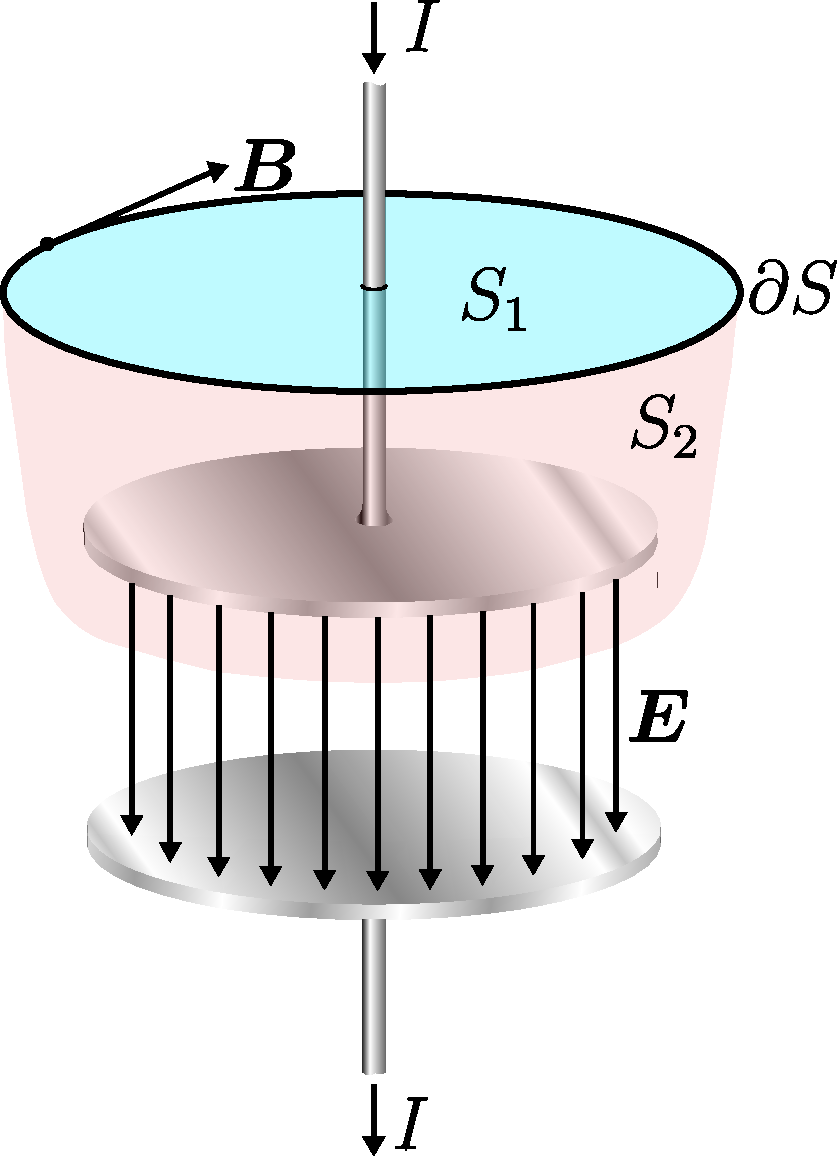
\includegraphics[height=0.55\textheight]{fig/lec02/Displacement_current_in_capacitor.pdf}
				\caption{Surfaces $S_1$ and $S_2$ share the same bounding contour $\partial S$. However, $S_1$ is pierced by conduction current, while $S_2$ is pierced by displacement current (adapted from: \href{https://commons.wikimedia.org/wiki/File:Displacement_current_in_capacitor.svg}{Wikimedia Commons}, public domain).}
			\end{figure}
		\end{column}
		\end{columns}
\end{frame}

%%%%%%%%%%%%%%%%%%%%%%%%%%%%%%%%%%%%%%%%%%%%%%%%%%%%%%%%%%%%%
%% The Ampere--Maxwell equation %%
%%%%%%%%%%%%%%%%%%%%%%%%%%%%%%%%%%%%%%%%%%%%%%%%%%%%%%%%%%%%%
\begin{frame}
	\frametitle{The Amp\`ere -- Maxwell equation}
	\begin{columns}
		\begin{column}{0.6\textwidth}
			The charge of capacitor is:
            $$Q = \oint_{S_2} \bm{D}\cdot \mathrm{d}\bm{S}.$$
            \onslide<2->{If the electric field ($\bm{D} = \varepsilon_0\varepsilon_\mathrm{r} \bm{E}$) changes, a displacement current results:
            $$I_{\mathrm{d}} = \frac{\mathrm{d}}{\mathrm{d} t} \oint_{S_2} \bm{D}\cdot \mathrm{d}\bm{S}$$}
            \begin{itemize}
                \item<3-> Is not a real current but a term to describe the changing electric field.
                \item<4-> Above, $\varepsilon_0$ is the vacuum permittivity and $\varepsilon_\mathrm{r}$ is the relative permittivity of a material.
            \end{itemize}
		\end{column}
        \hfill
		\begin{column}{0.4\textwidth}
			\begin{figure}
				\centering
				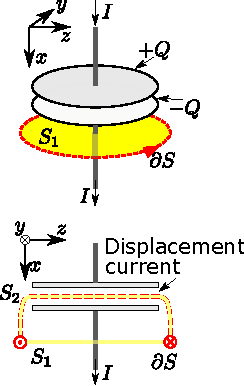
\includegraphics[height=0.65\textheight]{fig/lec02/Maxwell_integral_displacement_current.pdf}
				\caption{Illustration for calculation the displacement current (adapted from: \href{https://commons.wikimedia.org/wiki/File:Maxwell_integral_displacement_current.svg}{Wikimedia Commons}, public domain).}
			\end{figure}
		\end{column}
		\end{columns}
\end{frame}

%%%%%%%%%%%%%%%%%%%%%%%%%%%%%%%%%%%%%%%%%%%%%%%%%%%%%%%%%%%%%
%% The Ampere--Maxwell equation (cont.)%%
%%%%%%%%%%%%%%%%%%%%%%%%%%%%%%%%%%%%%%%%%%%%%%%%%%%%%%%%%%%%%
\begin{frame}
	\frametitle{The Amp\`ere -- Maxwell equation (cont.)}
        Adding the displacement current to \eqref{eq:ampere_law} we receive the Amp\`ere -- Maxwell equation:
            \begin{align}    
            \mbox{Integral form:} \quad  &\int_{\partial S} \bm{H} \cdot \mathrm{d}\bm{s} = \iint_{S}\left(\bm{J}_\mathrm{f} + \frac{\mathrm{d}}{\mathrm{d} t} \bm{D} \right)\cdot\mathrm{d}\bm{S}, \\
            \mbox{Differential form:} \quad &\nabla \times \bm{H} = \bm{J}_\mathrm{f} +  \frac{\partial\bm{D}}{\partial t}. 
            \label{eq:ampere_maxwell_law}
        \end{align}
        Above, $\bm{D}$ is the electric displacement field.
        \vspace{0.5cm}
        \begin{itemize}
            \item SI-unit: $[D] = \si{\coulomb\per\metre\squared}$
            \item SI-unit: $[E] = \si{\volt\per\metre}$
            \item $\varepsilon_0 \approx \SI{8.854e-12}{\farad\per\metre}$
        \end{itemize}
\end{frame}

%%%%%%%%%%%%%%%%%%%%%%%%%%%%%%%%%%%%%%%%%%%%%%%%%%%%%%%%%%%%%
%% Ampere's circuital law: magnetic flux %%
%%%%%%%%%%%%%%%%%%%%%%%%%%%%%%%%%%%%%%%%%%%%%%%%%%%%%%%%%%%%%
\begin{frame}
	\frametitle{Magnetic flux and flux linkage}
	\begin{columns}
		\begin{column}{0.575\textwidth}
			The magnetic flux $\phi$ is the surface integral of the normal component of $\bm{B}$ over that surface:
            \begin{align}
                \phi = \iint_{S} \bm{B} \cdot \mathrm{d}\bm{S}. 
            \end{align}
            \onslide<2->{As there are no magnetic monopoles, the magnetic flux through a closed surface (which is covering a volume without holes) is always zero:
            \begin{align}
                \oint_{S} \bm{B} \cdot \mathrm{d}\bm{S} = 0.
            \end{align}}
            \onslide<3->{The flux linkage $\psi$ is the product of the magnetic flux $\phi$ and the number of turns $N$ of a coil:
            \begin{align}
                \psi = N  \phi.
            \end{align}}
		\end{column}
        \hfill
		\begin{column}{0.425\textwidth}
            \vspace{-0.4cm}
			\begin{figure}
				\centering
				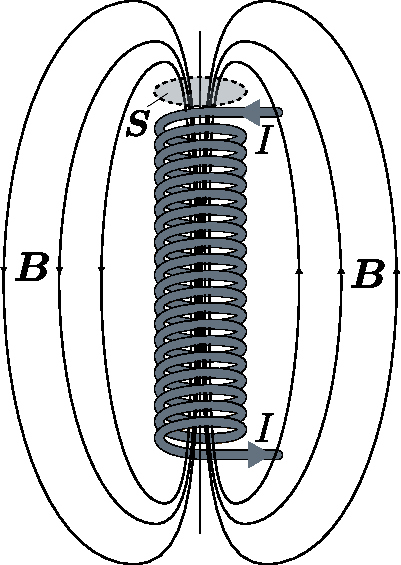
\includegraphics[height=0.68\textheight]{fig/lec02/Solenoid_Flux.pdf}
				\caption{Magnetic flux $\phi$ evaluated at the surface $\bm{S}$  (adapted from: \href{https://commons.wikimedia.org/wiki/File:Solenoid_and_Ampere_Law.png}{Wikimedia Commons}, Goodphy, \href{https://creativecommons.org/licenses/by-sa/4.0/deed.en}{CC BY-SA 4.0})}
                \label{fig:Solenoid_Flux}
			\end{figure}
		\end{column}
		\end{columns}
\end{frame}

%%%%%%%%%%%%%%%%%%%%%%%%%%%%%%%%%%%%%%%%%%%%%%%%%%%%%%%%%%%%%
%% Magnetic leakage flux %%
%%%%%%%%%%%%%%%%%%%%%%%%%%%%%%%%%%%%%%%%%%%%%%%%%%%%%%%%%%%%%
\begin{frame}
	\frametitle{Magnetic leakage flux}
	\begin{columns}
		\begin{column}{0.48\textwidth}
			\begin{itemize}
                \item In the scenarios with multiple coils, the magnetic flux generated by one coil will influence also the other coils.
                \item Exception: two coils are perfectly perpendicular to each other.
                \item However, the magnetic flux typically does not fully couple with the other coils
                \item The difference is the leakage flux $\phi_\sigma$.
            \end{itemize}
		\end{column}
        \hfill
		\begin{column}{0.48\textwidth}
            \vspace{-0.2cm}
			\begin{figure}
				\centering
				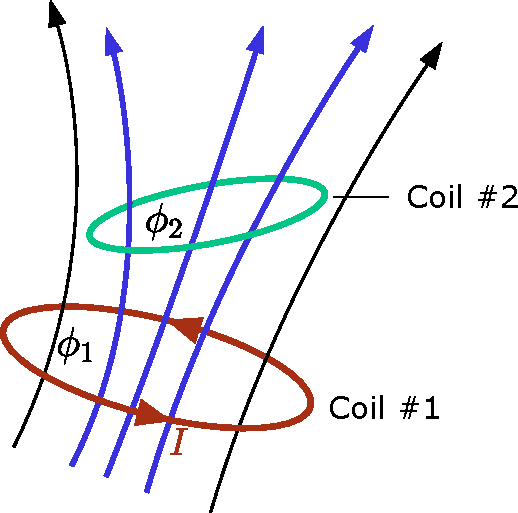
\includegraphics[height=0.55\textheight]{fig/lec02/Leakage_flux.pdf}
				\caption{The magnetic flux $\phi_1$ generated by the current $I$ does only partly couple with the second coil -- the difference $\phi_1-\phi_2$ is the leakage flux (adapted from: \href{https://commons.wikimedia.org/wiki/File:Mutual_Inductivity.svg}{Wikimedia Commons}, M. Wacenovsky, public domain)}
			\end{figure}
		\end{column}
		\end{columns}
\end{frame}

%%%%%%%%%%%%%%%%%%%%%%%%%%%%%%%%%%%%%%%%%%%%%%%%%%%%%%%%%%%%%
%% Inductance %%
%%%%%%%%%%%%%%%%%%%%%%%%%%%%%%%%%%%%%%%%%%%%%%%%%%%%%%%%%%%%%
\begin{frame}
	\frametitle{Inductance}
	The inductance $L$ describes the ratio between the magnetic flux linkage $\psi(t)$ to the current $i(t)$:
    \begin{align}
        \psi(t) = L i(t).
    \end{align}
    \textbf{Example}:  From the solenoid in \figref{fig:Solenoid_Flux} we know that the magnetic flux linkage $\psi$ is:
    $$\psi = N \iint_{S} \bm{B} \cdot \mathrm{d}\bm{S}= \frac{1}{l}N^2 \mu_0 I \pi r^2 $$
    with $r$ being the radius of the solenoid. Hence, the inductance $L$ is:
    $$L = \frac{\psi}{I} = \frac{N^2 \mu_0 \pi r^2}{l}.$$
    \begin{itemize}
        \item SI-unit: $[L] = \si{\henry} = \si{\volt\second\per\ampere}$
        \item The inductance is an important parameter describing inductive systems.
    \end{itemize}
\end{frame}

%%%%%%%%%%%%%%%%%%%%%%%%%%%%%%%%%%%%%%%%%%%%%%%%%%%%%%%%%%%%%
%% Self and mutual inductance %%
%%%%%%%%%%%%%%%%%%%%%%%%%%%%%%%%%%%%%%%%%%%%%%%%%%%%%%%%%%%%%
\begin{frame}
	\frametitle{Self and mutual inductance}
    \begin{columns}
		\begin{column}{0.45\textwidth}
            Based on the inductive coupling between the two coils from \figref{fig:Transformer3d_col3}, we can define the magnetic flux matrix:
            \begin{equation}
                \bm{\phi} = \begin{bmatrix} \phi_{11} & \phi_{12} \\ \phi_{21} & \phi_{22} \end{bmatrix} .
                \label{eq:flux_matrix_transformer}
            \end{equation}
            \vspace{-0.2cm}
			\begin{itemize}
                \item $\phi_{11}$: magnetic flux component of coil 1 due to its own current $i_1$
                \item $\phi_{12}$: magnetic flux component of coil 1 due to the current $i_2$ in coil 2
                \item $\phi_{21}$: magnetic flux component of coil 2 due to the current $i_1$ in coil 1
                \item $\phi_{22}$: magnetic flux component of coil 2 due to its own current $i_2$
            \end{itemize}
		\end{column}
        \hfill
		\begin{column}{0.525\textwidth}
			\begin{figure}
				\centering
				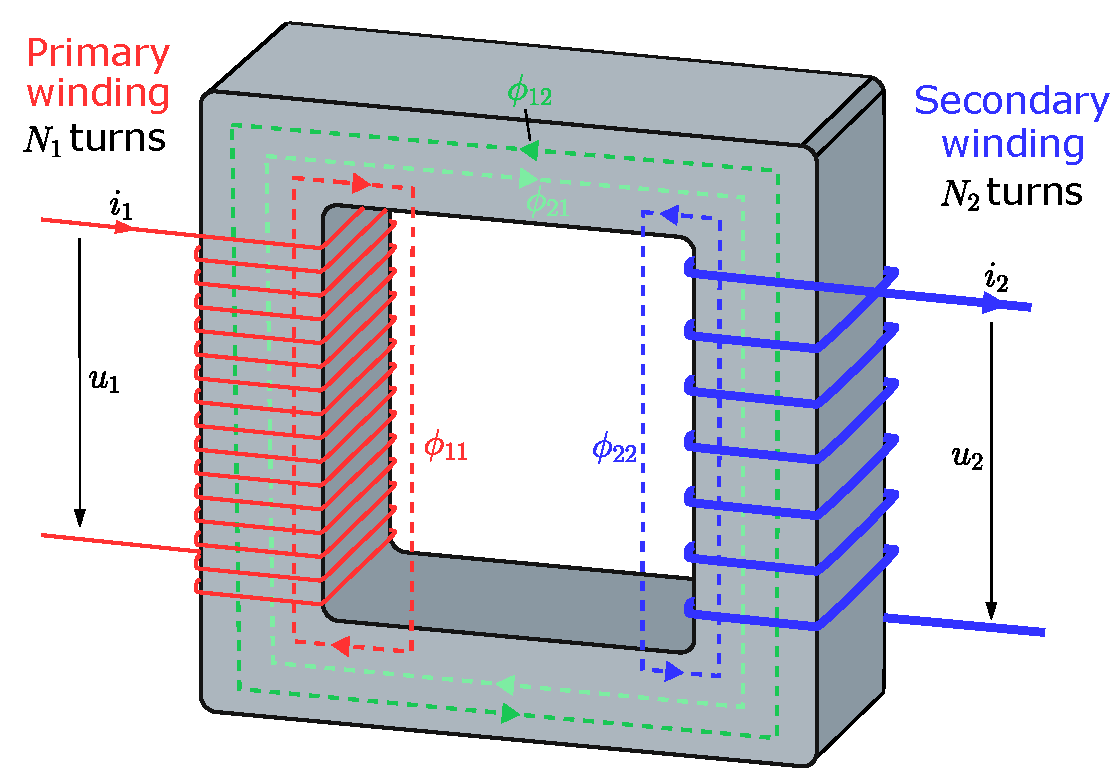
\includegraphics[height=0.575\textheight]{fig/lec02/Transformer3d_col3.pdf}
				\caption{Two coils coupled via a common core (adapted from: \href{https://commons.wikimedia.org/wiki/File:Transformer3d_col3.svg}{Wikimedia Commons}, Bill C., \href{https://creativecommons.org/licenses/by-sa/3.0/deed.en}{CC~BY-SA~3.0})}
                \label{fig:Transformer3d_col3}
			\end{figure}
		\end{column}
		\end{columns}
\end{frame}

%%%%%%%%%%%%%%%%%%%%%%%%%%%%%%%%%%%%%%%%%%%%%%%%%%%%%%%%%%%%%
%% Self and mutual inductance (cont.) %%
%%%%%%%%%%%%%%%%%%%%%%%%%%%%%%%%%%%%%%%%%%%%%%%%%%%%%%%%%%%%%
\begin{frame}
	\frametitle{Self and mutual inductance (cont.)}
    Utilizing the permeance definition (``magnetic conductance)'' 
    \begin{equation}
        \Lambda = \frac{\phi}{N i},
    \end{equation}
    we can represent \eqref{eq:flux_matrix_transformer} as:
    \begin{equation}
        \phi_{11} = \Lambda_{11} N_1 i_1, \quad \phi_{12} = \Lambda_{12} N_2 i_2, \quad \phi_{21} = \Lambda_{21} N_1 i_1, \quad \phi_{22} = \Lambda_{22} N_2 i_2.
    \end{equation}
    The resulting flux linkage per coil is then:
    \begin{equation}
        \begin{alignedat}{3}
        \psi_1 &= N_1\left(\phi_{11} + \phi_{21} + \phi_{12}\right), \quad && \psi_2 && =  N_2\left(\phi_{22} + \phi_{12} + \phi_{21}\right)\\
               &=\underbrace{\left(\Lambda_{11}N_1^2+\Lambda_{21}N_1^2\right)}_{L_1}i_1 + \underbrace{\Lambda_{12}N_1N_2}_{M_{12}}i_2, \quad && && =\underbrace{\left(\Lambda_{22}N_2^2+\Lambda_{12}N_1^2\right)}_{L_2}i_2 + \underbrace{\Lambda_{21}N_1N_2}_{M_{21}}i_1. 
        \end{alignedat}
        \label{eq:flux_linkage_transformer}
    \end{equation}
    Above, $L_1$ and $L_2$ are the self-inductances, $M_{12}$ and $M_{21}$ are the mutual inductances.
\end{frame}

%%%%%%%%%%%%%%%%%%%%%%%%%%%%%%%%%%%%%%%%%%%%%%%%%%%%%%%%%%%%%
%% Self and mutual inductance (cont.) %%
%%%%%%%%%%%%%%%%%%%%%%%%%%%%%%%%%%%%%%%%%%%%%%%%%%%%%%%%%%%%%
\begin{frame}
	\frametitle{Self and mutual inductance (cont.)}
    Hence, we can define the flux linkages of both coils using the following inductance matrix:
    \begin{equation}
        \bm{\psi} = \begin{bmatrix} \psi_1 \\ \psi_2 \end{bmatrix} = \begin{bmatrix} L_1 & M_{12} \\ M_{21} & L_2 \end{bmatrix} \begin{bmatrix} i_1 \\ i_2 \end{bmatrix}.
    \end{equation}
    Due to the symmetry of the inductive coupling, the mutual inductances are identical:
    \begin{equation}
        M_{12} = M_{21} = M.
    \end{equation}
    Based on \eqref{eq:flux_linkage_transformer}, we can also split the self-inductances into the sum of the inductance of the coil itself (magnetic leakage) and the mutual inductance:
    \begin{equation}
        L_i = L_{i\sigma} + M. 
    \end{equation}
    Finally, we can define the coupling coefficient $k$ as:
    \begin{equation}
        k = \frac{M}{\sqrt{L_1 L_2}}, \qquad 0 \leq k \leq 1,
    \end{equation}
    which indicates the degree of inductive coupling between the coils.
\end{frame}

%%%%%%%%%%%%%%%%%%%%%%%%%%%%%%%%%%%%%%%%%%%%%%%%%%%%%%%%%%%%%
%% Boosting the magnet field with ferromagnetic materials %%
%%%%%%%%%%%%%%%%%%%%%%%%%%%%%%%%%%%%%%%%%%%%%%%%%%%%%%%%%%%%%
\begin{frame}
	\frametitle{Boosting the magnet field with ferromagnetic materials}
	\begin{columns}
		\begin{column}{0.575\textwidth}
			While $\bm{H}$ depends on the currents applied to an object, $\bm{B}$ depends on the material properties of the object. In free space (vacuum), the relation is linear and represented by the magnetic constant $\mu_0$:
            \begin{align}
                \bm{B} = \mu_0 \bm{H} \quad \mbox{with} \quad \mu_0 \approx \SI{4 \pi e-7}{\newton\per\ampere\squared}.
            \end{align}
            \onslide<2->{To boost $\bm{B}$ for a given $\bm{H}$, ferromagnetic materials are typically used. These materials have a high relative magnetic permeability $\mu_{\mathrm{r}}$:
            \begin{align}
                \bm{B} = \mu \bm{H} = \mu_0 \mu_{\mathrm{r}} \bm{H}.
                \label{eq:linear_permeability} 
            \end{align}}
            \onslide<3->{Note that $\mu_{\mathrm{r}}$ is a dimensionless quantity and that \eqref{eq:linear_permeability} assumes linear and isotropic material behavior.}
		\end{column}
        \hfill
		\begin{column}{0.425\textwidth}
            \vspace{-0.2cm}
			\begin{figure}
				\centering
				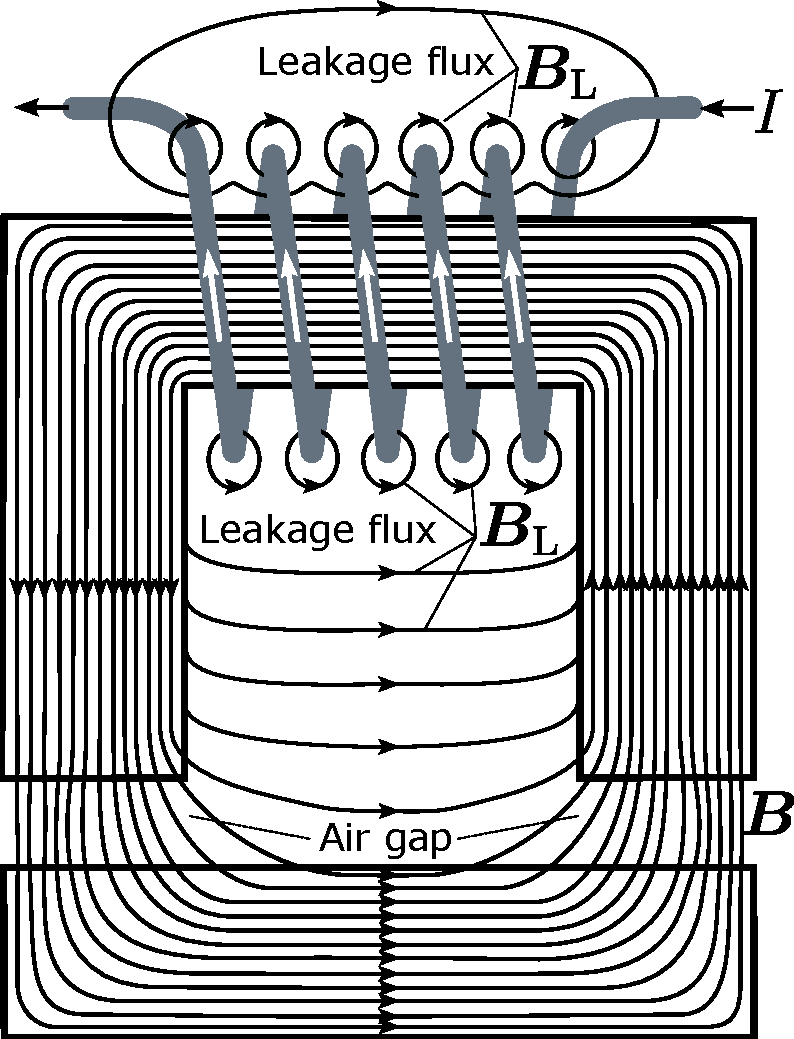
\includegraphics[height=0.68\textheight]{fig/lec02/Electromagnet_with_gap.pdf}
				\caption{Simplified magnetic field lines of an iron yoke with a coil  (adapted from: \href{https://en.m.wikipedia.org/wiki/File:Electromagnet_with_gap.svg}{Wikimedia Commons}, public domain)}
			\end{figure}
		\end{column}
		\end{columns}
\end{frame}

%%%%%%%%%%%%%%%%%%%%%%%%%%%%%%%%%%%%%%%%%%%%%%%%%%%%%%%%%%%%%
%% Relative permeability and magnetic saturation %%
%%%%%%%%%%%%%%%%%%%%%%%%%%%%%%%%%%%%%%%%%%%%%%%%%%%%%%%%%%%%%
\begin{frame}
	\frametitle{Relative permeability and magnetic saturation}
	\begin{columns}
		\begin{column}{0.575\textwidth}
			\begin{table}
            \centering
            \begin{tabular}{lc}
                \toprule
                Material & $\mu_{\mathrm{r}}$ (range)\\
                \midrule
                Air / copper / aluminum & $(\approx)$1 \\ 
                Iron (99.8\,\% pure) & 5000\\
                Electrical steel & 2000 - 35000\\
                Ferrite & 200 - 20000\\
                \bottomrule
            \end{tabular}
            \caption{Typical relative permeabilities of materials}
            \label{tab:rel_permeabilities}
            \end{table}
        \onslide<2->{Linear magnetic behavior ($\mu_{\mathrm{r}}=\mbox{const.}$) is only a local approximation. When considering larger $H$ ranges, the (differential) permeability becomes nonlinear:
        \begin{align}
            \mu_\mathrm{r}(H) =  \frac{\mathrm{d}B}{\mathrm{d}H}.
        \end{align}}
		\end{column}
        \hfill
		\begin{column}{0.425\textwidth}
            \onslide<2->
			\begin{figure}
				\centering
				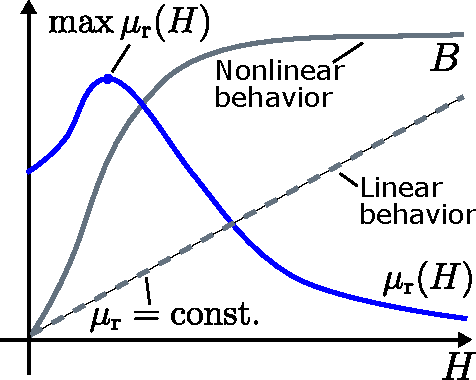
\includegraphics[height=0.5\textheight]{fig/lec02/Permeability_of_ferromagnet.pdf}
				\caption{Illustrative magnetization curves for ferromagnets (and ferrimagnets) and corresponding permeabilities  (adapted from: \href{https://commons.wikimedia.org/wiki/File:Permeability_of_ferromagnet_by_Zureks.svg}{Wikimedia Commons}, public domain)}
			\end{figure}
		\end{column}
		\end{columns}
\end{frame}


%%%%%%%%%%%%%%%%%%%%%%%%%%%%%%%%%%%%%%%%%%%%%%%%%%%%%%%%%%%%%
%% Magnetic domains (1) %%
%%%%%%%%%%%%%%%%%%%%%%%%%%%%%%%%%%%%%%%%%%%%%%%%%%%%%%%%%%%%%
\begin{frame}
	\frametitle{Magnetic domains (1)}
    \begin{columns}
	\begin{column}{0.48\textwidth}
    \begin{itemize}
        \item Magnetic domains are regions within a material where the magnetic moments of atoms are aligned (``mini magnets'').
        \item The magnetization within each domain points in a uniform direction, but the magnetization of different domains may point in different directions.
    \end{itemize}
    \end{column}
    \hfill
    \begin{column}{0.52\textwidth}
        \onslide<2->{\begin{figure}
            \centering
            \movie{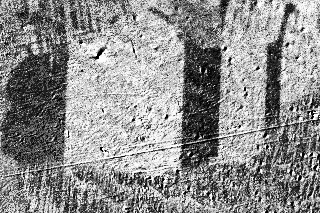
\includegraphics[height=0.3\textheight]{fig/lec02/Moving_magnetic_domains_preview.png}}{fig/lec02/Moving_magnetic_domains.gif}
            \caption{Animation of moving domain walls (source: \href{https://commons.wikimedia.org/wiki/File:Moving_magnetic_domains_by_Zureks.gif}{Wikimedia Commons}, Zureks, \href{https://creativecommons.org/licenses/by-sa/3.0/deed.en}{CC BY-SA 3.0})}
        \end{figure}}
    \end{column}
\end{columns}
\begin{figure}
\begin{columns}
	\begin{column}{0.6\textwidth}
            \centering
            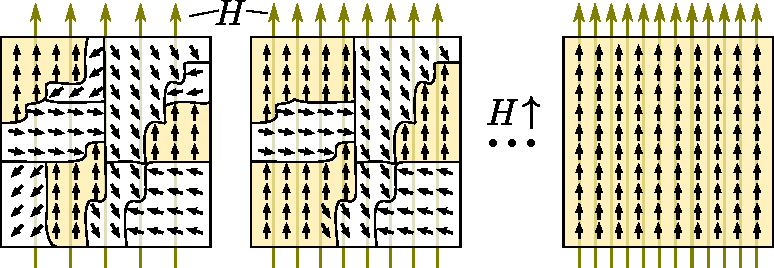
\includegraphics[width=0.9\textwidth]{fig/lec02/Growing-magnetic-domains.pdf}
    \end{column}
    \begin{column}{0.35\textwidth}
        \caption{\raggedright Change of magnetic domains due to an external magnetic field  (adapted from: \href{https://de.wikipedia.org/wiki/Datei:Growing-magnetic-domains.svg}{Wikimedia Commons}, M. Run, \href{https://creativecommons.org/licenses/by-sa/4.0/deed.en}{CC BY-SA 4.0})}
    \end{column}
\end{columns}
\end{figure}
\end{frame}

%%%%%%%%%%%%%%%%%%%%%%%%%%%%%%%%%%%%%%%%%%%%%%%%%%%%%%%%%%%%%
%% Magnetic domains (2) %%
%%%%%%%%%%%%%%%%%%%%%%%%%%%%%%%%%%%%%%%%%%%%%%%%%%%%%%%%%%%%%
\begin{frame}
	\frametitle{Magnetic domains (2)}
    \begin{itemize}
        \item A large region of material with a constant magnetization throughout creates a large magnetic field (diagram a) below). This requires a lot of magnetostatic energy stored in the field. 
        \item<2-> To reduce this energy, the sample can ``split'' into two domains, with the magnetization in opposite directions in each domain which reduces the overall field (diagram b) below).
        \item<3->  To reduce the field energy further, each of these domains can split also, resulting in smaller parallel domains with magnetization in alternating directions, with smaller amounts of field outside the material (diagram c) below).
    \end{itemize}
\begin{figure}
\begin{columns}
	\begin{column}{0.55\textwidth}
            \centering
            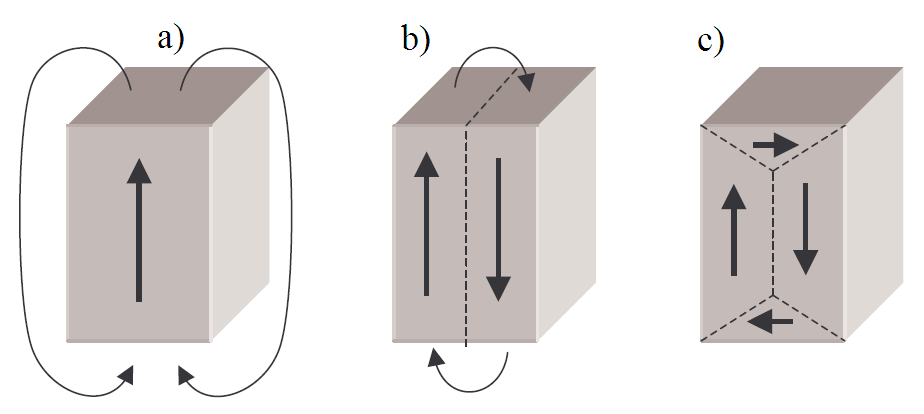
\includegraphics[width=0.8\textwidth]{fig/lec02/Magnetic_domains_energy_min.png}
    \end{column}
    \begin{column}{0.4\textwidth}
        \caption{\raggedright Simplified representation of the formation of magnetic domains on the basis of energy minimization  (source: \href{https://commons.wikimedia.org/wiki/File:Powstawanie_domen_by_Zureks.png}{Wikimedia Commons}, public domain)}
    \end{column}
\end{columns}
\end{figure}
\end{frame}

%%%%%%%%%%%%%%%%%%%%%%%%%%%%%%%%%%%%%%%%%%%%%%%%%%%%%%%%%%%%%
%% Hysteresis %%
%%%%%%%%%%%%%%%%%%%%%%%%%%%%%%%%%%%%%%%%%%%%%%%%%%%%%%%%%%%%%
\begin{frame}
	\frametitle{Hysteresis}
	\begin{columns}
		\begin{column}{0.575\textwidth}
            \begin{itemize}
                \item Material defects lead to small, random jumps in magnetization called Barkhausen jumps.
                \item Domain walls move irregularly.
                \item<2-> Process also depends on the history of the magnetization process (dynamic system).
            \end{itemize}
			\begin{figure}
                \centering
                \movie{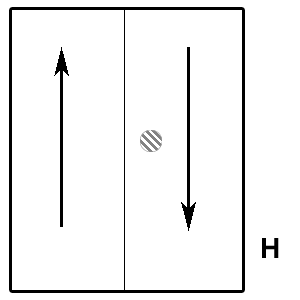
\includegraphics[height=0.3\textheight]{fig/lec02/Barkhausen_jump_preview.png}}{fig/lec02/Barkhausen_jump.gif}
                \caption{Animation of the Barkhausen jump (source: \href{https://commons.wikimedia.org/wiki/File:Barkhausensprung.gif}{Wikimedia Commons},  public domain)}
            \end{figure}
		\end{column}
        \hfill
		\begin{column}{0.425\textwidth}
            \vspace{-0.2cm}
			\onslide<2->\begin{figure}
				\centering
				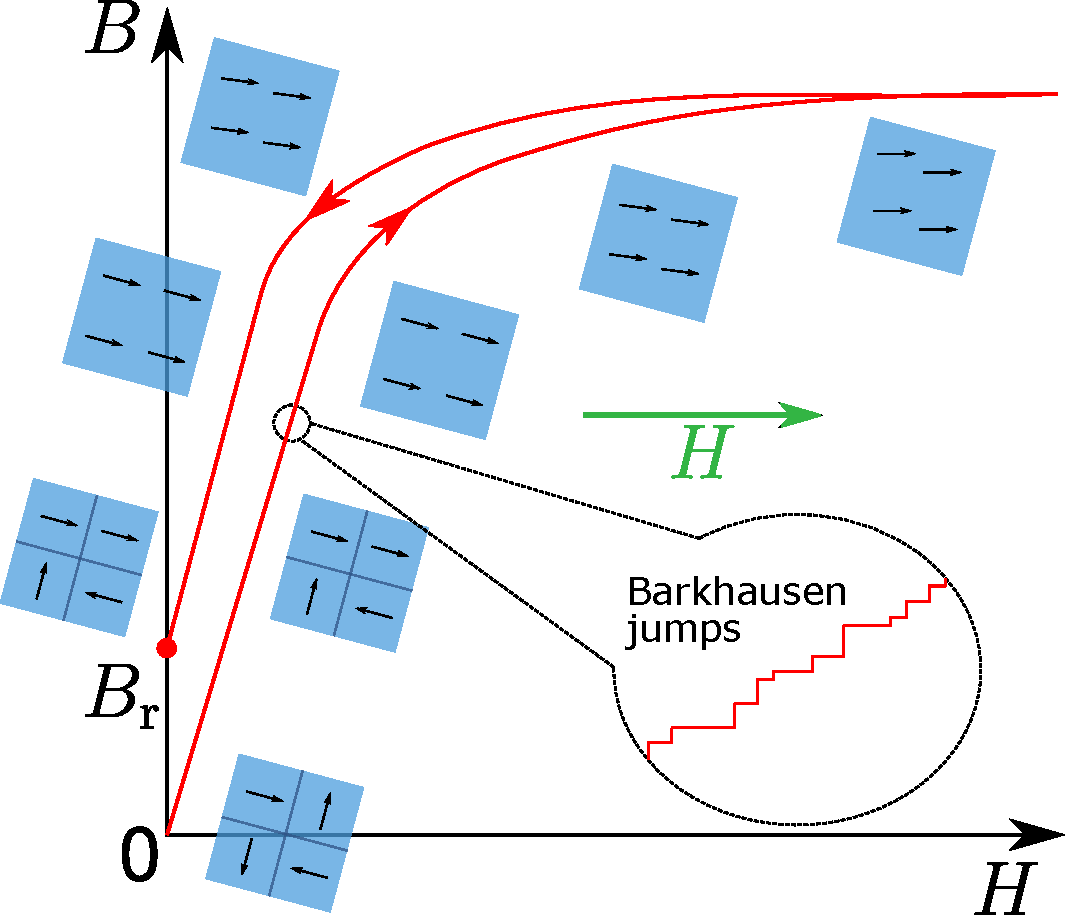
\includegraphics[height=0.5\textheight]{fig/lec02/Ferromagnet_magnetization_and_magnetic_domains_and_hysteresis.pdf}
				\caption{Simplified hysteresis curve in first quadrant with magnetic domains illustration (adapted from: \href{https://commons.wikimedia.org/wiki/File:Ferromagnet_magnetization_and_magnetic_domains_and_hysteresis.svg}{Wikimedia Commons}, Fralama, \href{https://creativecommons.org/licenses/by-sa/3.0/deed.enn}{CC BY-SA 3.0})}
			\end{figure}
		\end{column}
		\end{columns}
\end{frame}

%%%%%%%%%%%%%%%%%%%%%%%%%%%%%%%%%%%%%%%%%%%%%%%%%%%%%%%%%%%%%
%% Hysteresis curve and losses %%
%%%%%%%%%%%%%%%%%%%%%%%%%%%%%%%%%%%%%%%%%%%%%%%%%%%%%%%%%%%%%
\begin{frame}
	\frametitle{Hysteresis curve and losses}
	\begin{columns}
		\begin{column}{0.5\textwidth}
            \begin{itemize}
                \item With an external and varying field $H$, a closed hysteresis curve is obtained.
                \item<2-> Traversing through the curve requires to move the domain walls and rotate the elementary magnets within the domains.
                \item<3-> This process requires work and leads to heat dissipation (losses).
                \item<4-> The area enclosed by the hysteresis curve is identical to the relative remagnetization work (per volume, that is, $[w_{\mathrm{h}}]=\si{\joule\per\metre\cubed}$):
            \end{itemize}
            \onslide<4->{\begin{align}
                w_{\mathrm{h}} = \oint \bm{H} \cdot \mathrm{d}\bm{B}.
            \end{align}}
		\end{column}
        \hfill
		\begin{column}{0.475\textwidth}
            \vspace{-0.2cm}
			\begin{figure}
				\centering
				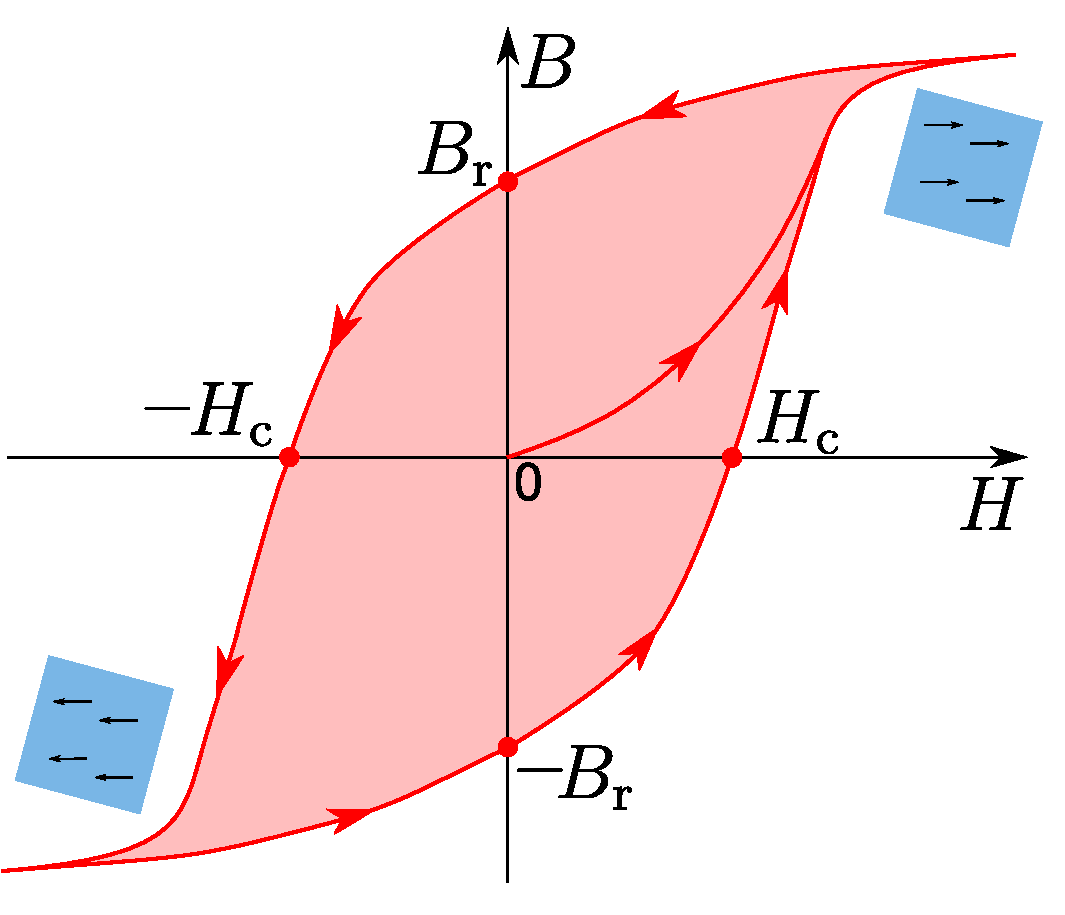
\includegraphics[height=0.55\textheight]{fig/lec02/Hyteresis_curve_full.pdf}
				\caption{Exemplary hysteresis curve with $B_\mathrm{r}$ being the remanence field density and $H_\mathrm{c}$ the coercivity field strength}
			\end{figure}
		\end{column}
		\end{columns}
\end{frame}

%%%%%%%%%%%%%%%%%%%%%%%%%%%%%%%%%%%%%%%%%%%%%%%%%%%%%%%%%%%%%
%% How can we model the hysteresis losses? %%
%%%%%%%%%%%%%%%%%%%%%%%%%%%%%%%%%%%%%%%%%%%%%%%%%%%%%%%%%%%%%
\begin{frame}
	\frametitle{How can we model the hysteresis losses?}
	\begin{columns}
		\begin{column}{0.5\textwidth}
            \vspace{-0.15cm}
            \begin{enumerate}
                \item \textbf{Data look-up table:} Measure the hysteresis curve and its losses directly on a test bench (cf. \href{https://www.princeton.edu/~minjie/magnet.html}{MagNet project data hub}).
                \item<2-> \textbf{Loss-fitted models:} Use empirical models to fit the hysteresis losses (e.g., Steinmetz model):
                $$P_{\mathrm{h}} = k_{\mathrm{h}}f^a \max\{B\}^b.$$
                \item<3-> \textbf{Curve-fitted models:} Use empirical models to describe the hysteresis curve and derive the losses (e.g., ODE as in the Jiles-Atherton model):
                $$\frac{\mathrm{d}B}{\mathrm{d}H} = f(B,H).$$
            \end{enumerate}
		\end{column}
        \hfill
		\begin{column}{0.475\textwidth}
            \vspace{-0.2cm}
			\begin{figure}
				\centering
				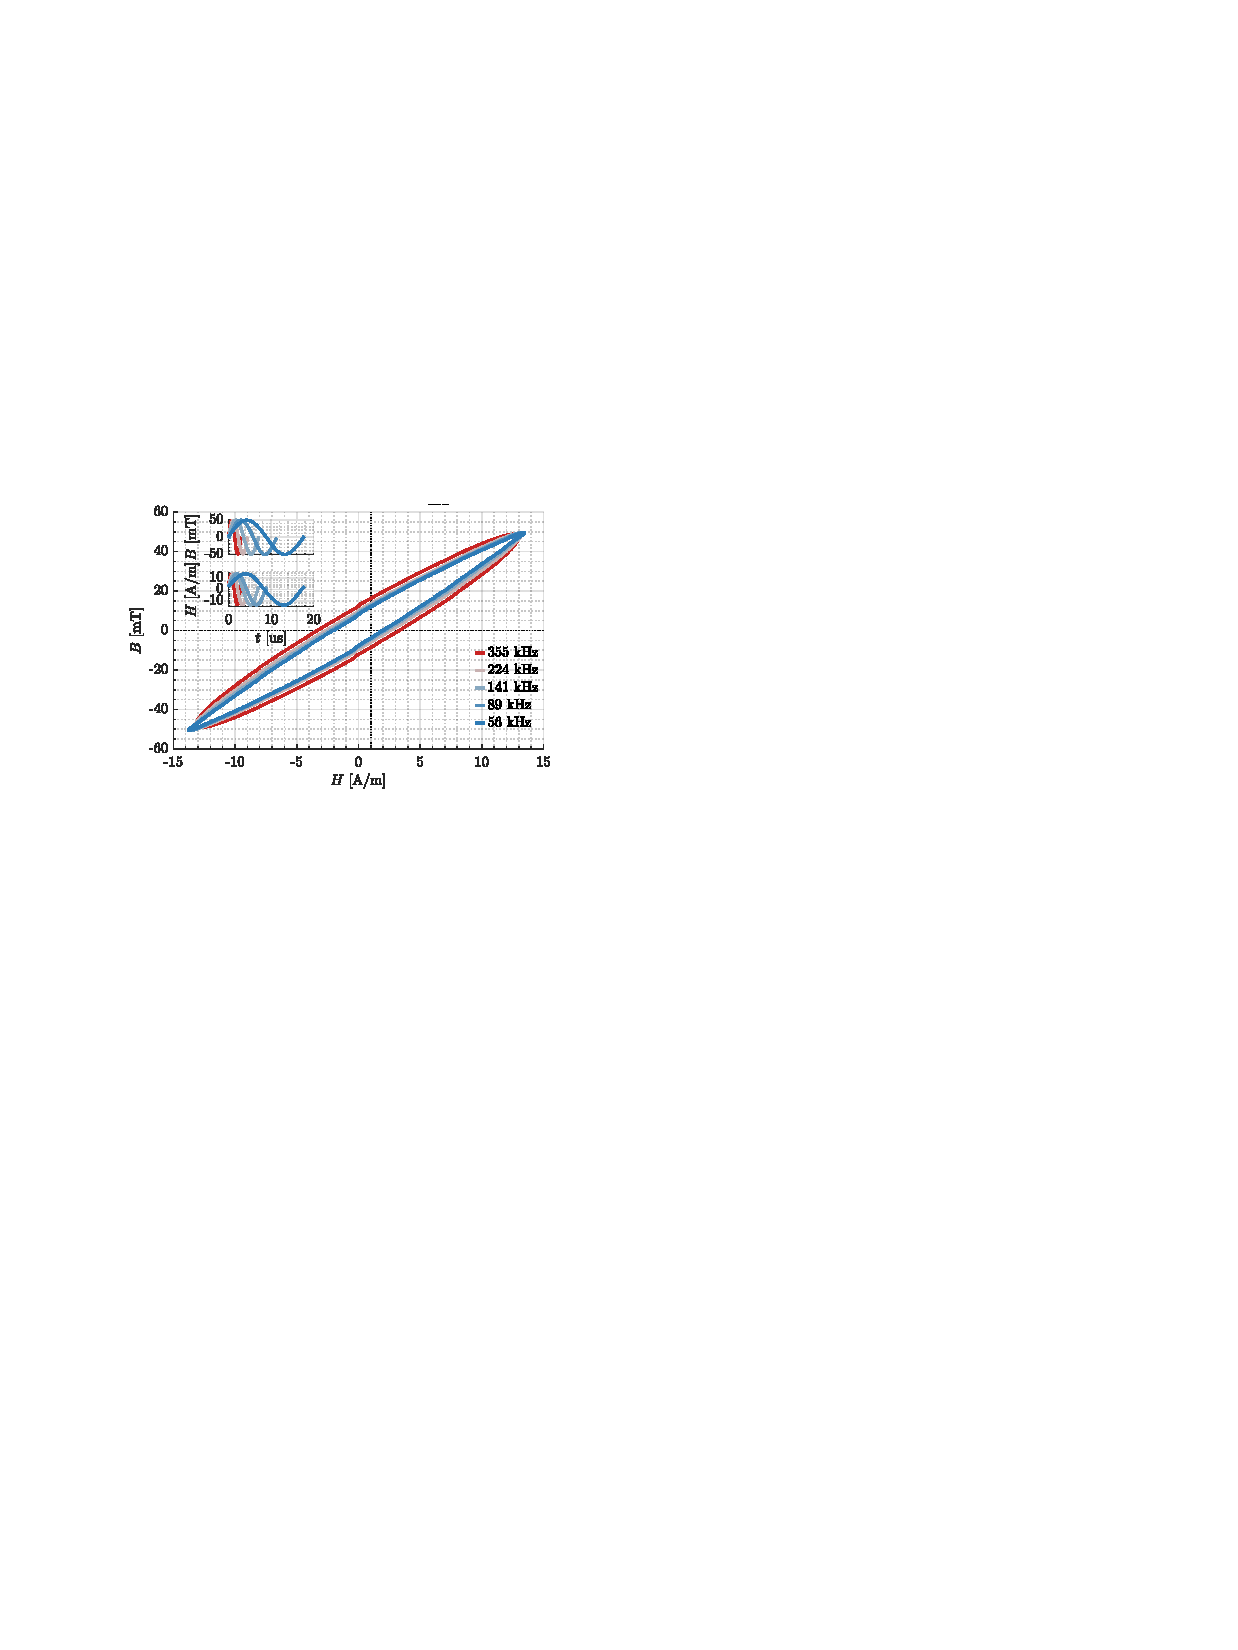
\includegraphics[height=0.55\textheight]{fig/lec02/Hysteresis_curve_Serrano_et_al.pdf}
				\caption{Measured $B$-$H$ loops for sinusoidal excitation at different frequencies (source: \href{https://ieeexplore.ieee.org/abstract/document/10169101}{IEEE TPEL}, Serrano et al., \href{https://creativecommons.org/licenses/by/4.0/}{CC BY 4.0})}
			\end{figure}
		\end{column}
		\end{columns}
\end{frame}

%%%%%%%%%%%%%%%%%%%%%%%%%%%%%%%%%%%%%%%%%%%%%%%%%%%%%%%%%%%%%
%% Alternative to boost the magnet field: permanent magnets %%
%%%%%%%%%%%%%%%%%%%%%%%%%%%%%%%%%%%%%%%%%%%%%%%%%%%%%%%%%%%%%
\begin{frame}
	\frametitle{Alternative to boost the magnet field: permanent magnets (PMs)}
    \begin{columns}
        \begin{column}{0.48\textwidth}
        \begin{itemize}
            \item Create own persistent magnetic fields.
            \item Consist of hard ferromagnetic (or ferrimagnetic) materials.
            \item<2-> Nearly constant magnetiziation offset $\bm{B}_\mathrm{PM}$ in the usual operating range:
            \onslide<2->{\begin{align}
                \bm{B} = \mu_0 \mu_{\mathrm{r}} \bm{H} \approx \mu_0 \bm{H} + \bm{B}_\mathrm{PM}.
            \end{align}}
        \end{itemize}
        \end{column}
        \hfill
        \begin{column}{0.4\textwidth}
            \begin{figure}
                \centering
                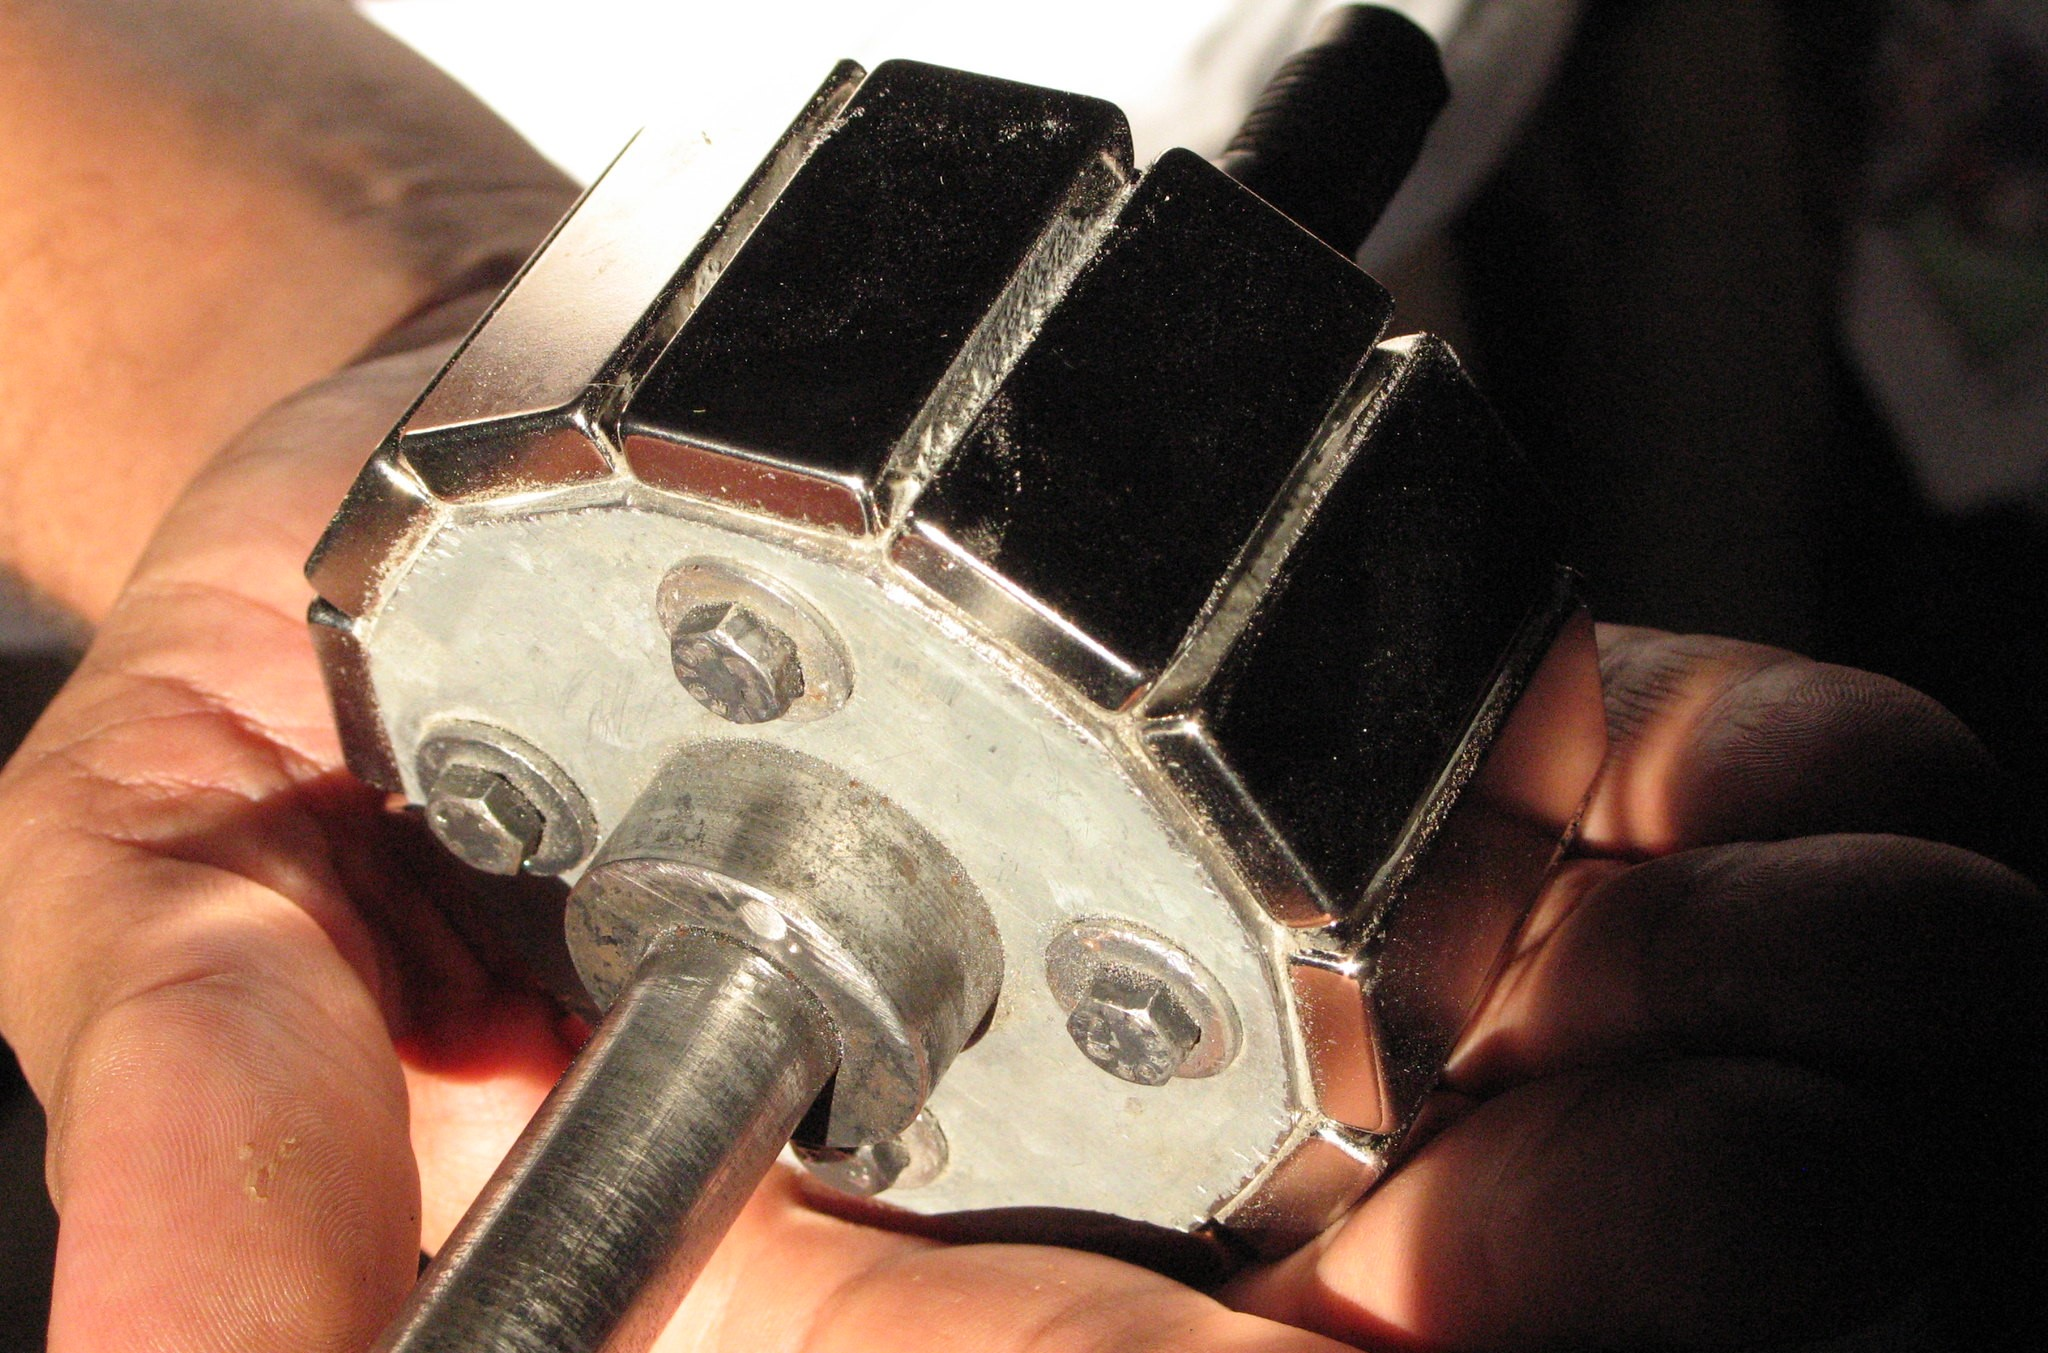
\includegraphics[width=0.65\textwidth]{fig/lec02/PM_rotor_example.jpg}
                \caption{PMs on a rotor (source: \href{https://www.flickr.com/photos/aidg/2382339376}{flickr.com}, AIDG, \href{https://creativecommons.org/licenses/by-nc-sa/2.0/}{CC BY-NC-SA 2.0})}
            \end{figure}
        \end{column}
    \end{columns}
    \begin{figure}
    \begin{columns}
        \begin{column}{0.6\textwidth}
                \centering
                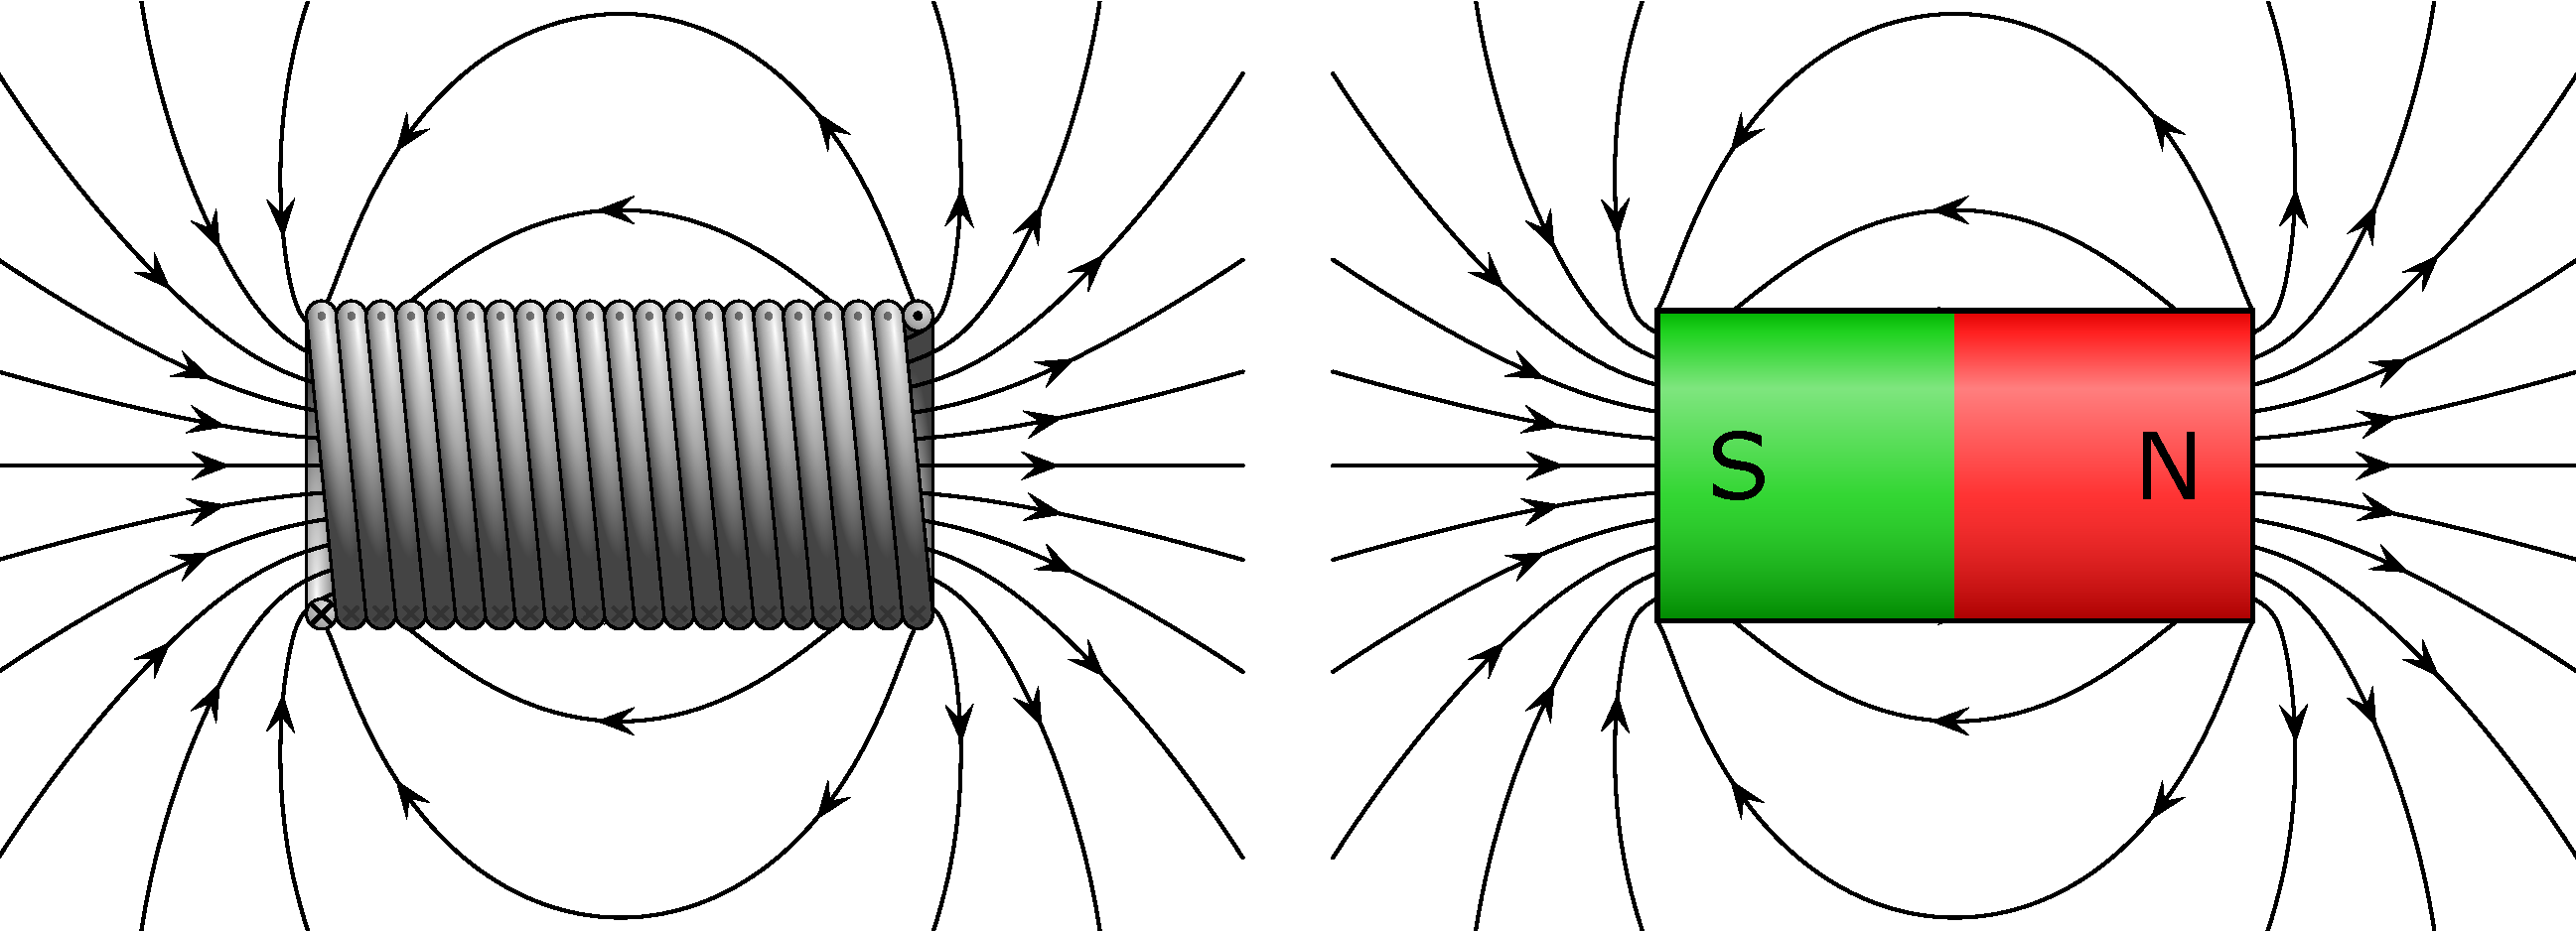
\includegraphics[width=0.9\textwidth]{fig/lec02/Coil_magnet_comparison.pdf}
        \end{column}
        \begin{column}{0.35\textwidth}
            \caption{\raggedright Permanent magnets as alternatives to current-based excitation  (source: \href{https://commons.wikimedia.org/wiki/File:VFPt_cylindrical_tightly-wound_coil-and-bar-magnet-comparison.svg}{Wikimedia Commons}, M. Run, \href{https://creativecommons.org/licenses/by-sa/3.0/deed.en}{CC BY-SA 3.0})}
        \end{column}
    \end{columns}
    \end{figure}
    \end{frame}

%%%%%%%%%%%%%%%%%%%%%%%%%%%%%%%%%%%%%%%%%%%%%%%%%%%%%%%%%%%%%
%% Hyteresis curve of permanent magnets %%
%%%%%%%%%%%%%%%%%%%%%%%%%%%%%%%%%%%%%%%%%%%%%%%%%%%%%%%%%%%%%
\begin{frame}
	\frametitle{Hyteresis curve of permanent magnets}
	\begin{columns}
		\begin{column}{0.45\textwidth}
            \begin{itemize}
                \item PM's magnetization is nearly  completely saturated and constant in common operation area.
                \item<2-> The greater the coercivity $H_\mathrm{c}$, the greater the resistance of the PM to demagnetization by external fields.
                \item<3-> Beyond the so-called knee point, PMs are (partially) demagnetized.
                \item<4-> Important figure of merit is the so-called energy product:
                \begin{align}
                    \onslide<4->{(BH)_{\max} = \max \left\{- B H \right\}.}
                \end{align}
                \item<5-> The higher $(BH)_{\max}$ the less PM material is needed for an application.
            \end{itemize}
		\end{column}
        \hfill
		\begin{column}{0.42\textwidth}
            \vspace{-0.2cm}
			\begin{figure}
				\centering
				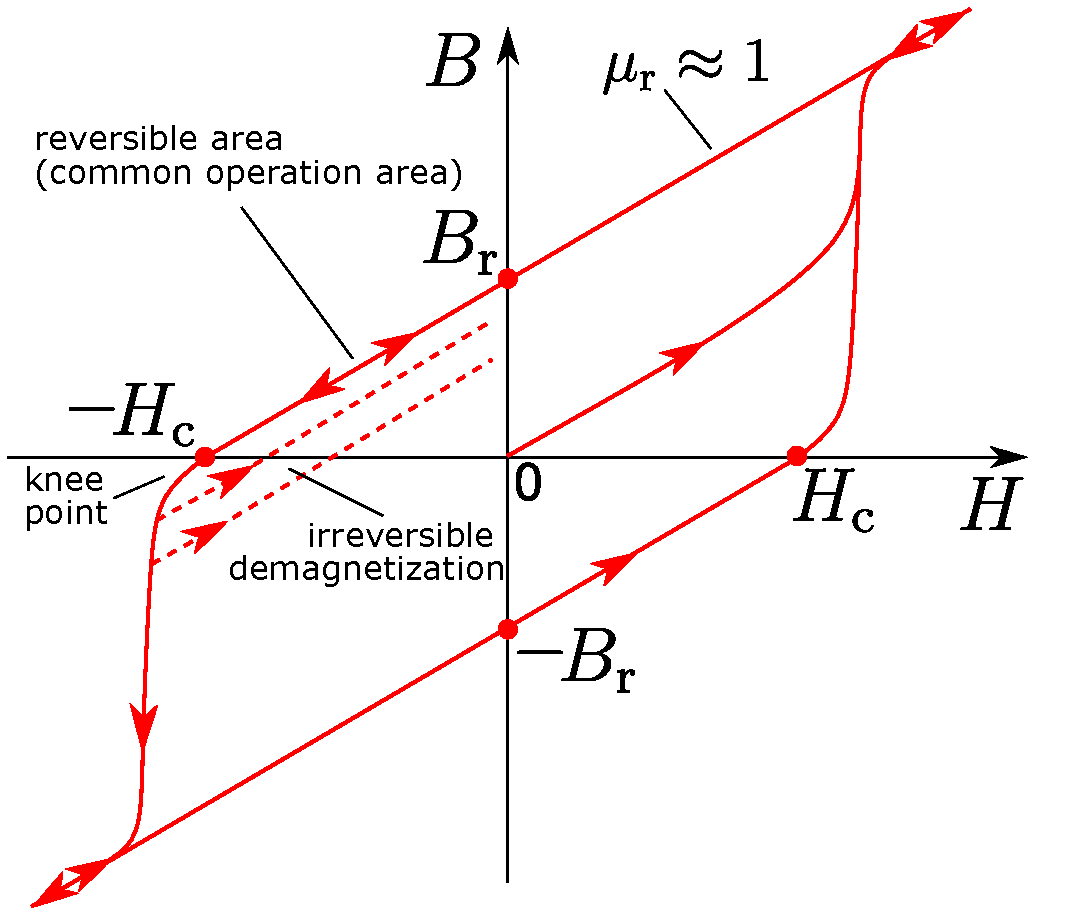
\includegraphics[height=0.6\textheight]{fig/lec02/Hyteresis_curve_PM.pdf}
				\caption{Exemplary hysteresis curve of a permanent magnet}
			\end{figure}
		\end{column}
		\end{columns}
\end{frame}

%%%%%%%%%%%%%%%%%%%%%%%%%%%%%%%%%%%%%%%%%%%%%%%%%%%%%%%%%%%%%
%% Hyteresis curve of permanent magnets (temperature dependence) %%
%%%%%%%%%%%%%%%%%%%%%%%%%%%%%%%%%%%%%%%%%%%%%%%%%%%%%%%%%%%%%
\begin{frame}
	\frametitle{Hyteresis curve of permanent magnets (temperature dependence)}
	\begin{columns}
		\begin{column}{0.4\textwidth}
            \begin{itemize}
                \item Besides pressure and vibrations, PMs are also sensitive to temperature.
                \item The coercivity $H_\mathrm{c}$ and the remanence $B_\mathrm{r}$ decrease with increasing temperature.
                \item Hence, with higher temperatures, a PM gets more susceptible to demagnetization.
            \end{itemize}
		\end{column}
        \hspace{0.25cm}
		\begin{column}{0.4\textwidth}
			\begin{figure}
				\centering
				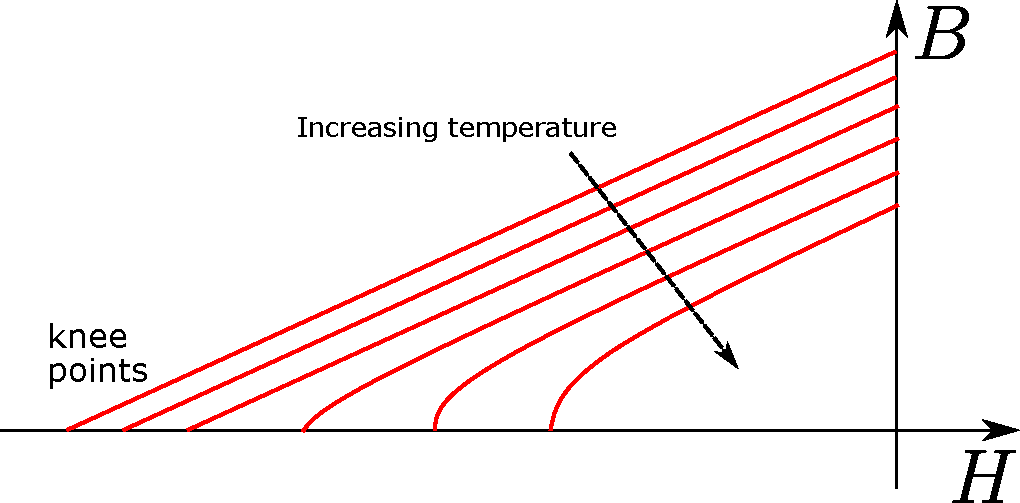
\includegraphics[height=0.4\textheight]{fig/lec02/Hyteresis_curve_PM_temperature.pdf}
				\caption{Qualitative representation of the temperature dependence of permanent magnets}
			\end{figure}
		\end{column}
		\end{columns}
\end{frame}

%%%%%%%%%%%%%%%%%%%%%%%%%%%%%%%%%%%%%%%%%%%%%%%%%%%%%%%%%%%%%
%% Energy product overview of permanent magnets %%
%%%%%%%%%%%%%%%%%%%%%%%%%%%%%%%%%%%%%%%%%%%%%%%%%%%%%%%%%%%%%
\begin{frame}
	\frametitle{Energy product overview of permanent magnets}
        \begin{figure}
            \centering
            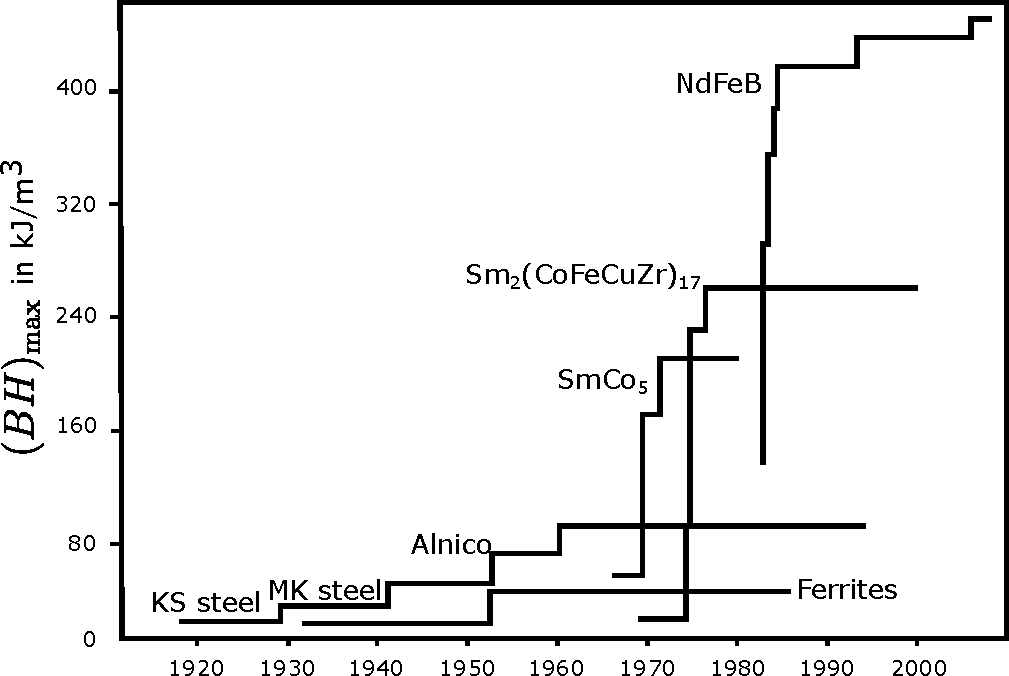
\includegraphics[height=0.65\textheight]{fig/lec02/PM_energy_product.pdf}
            \caption{Historic development of PM materials and their energy product (adapted from: \href{https://commons.wikimedia.org/wiki/File:Magnetische_Energiedichte.svg}{Wikimedia Commons}, Kopiersperre, \href{https://creativecommons.org/licenses/by-sa/4.0/deed.en}{CC BY-SA 4.0})}
        \end{figure}
\end{frame}


%%%%%%%%%%%%%%%%%%%%%%%%%%%%%%%%%%%%%%%%%%%%%%%%%%%%%%%%%%%%%
%% Manufacturing process of NdFeB permanent magnets %%
%%%%%%%%%%%%%%%%%%%%%%%%%%%%%%%%%%%%%%%%%%%%%%%%%%%%%%%%%%%%%
\begin{frame}
	\frametitle{Manufacturing process of NdFeB permanent magnets}
        \begin{figure}
            \centering
            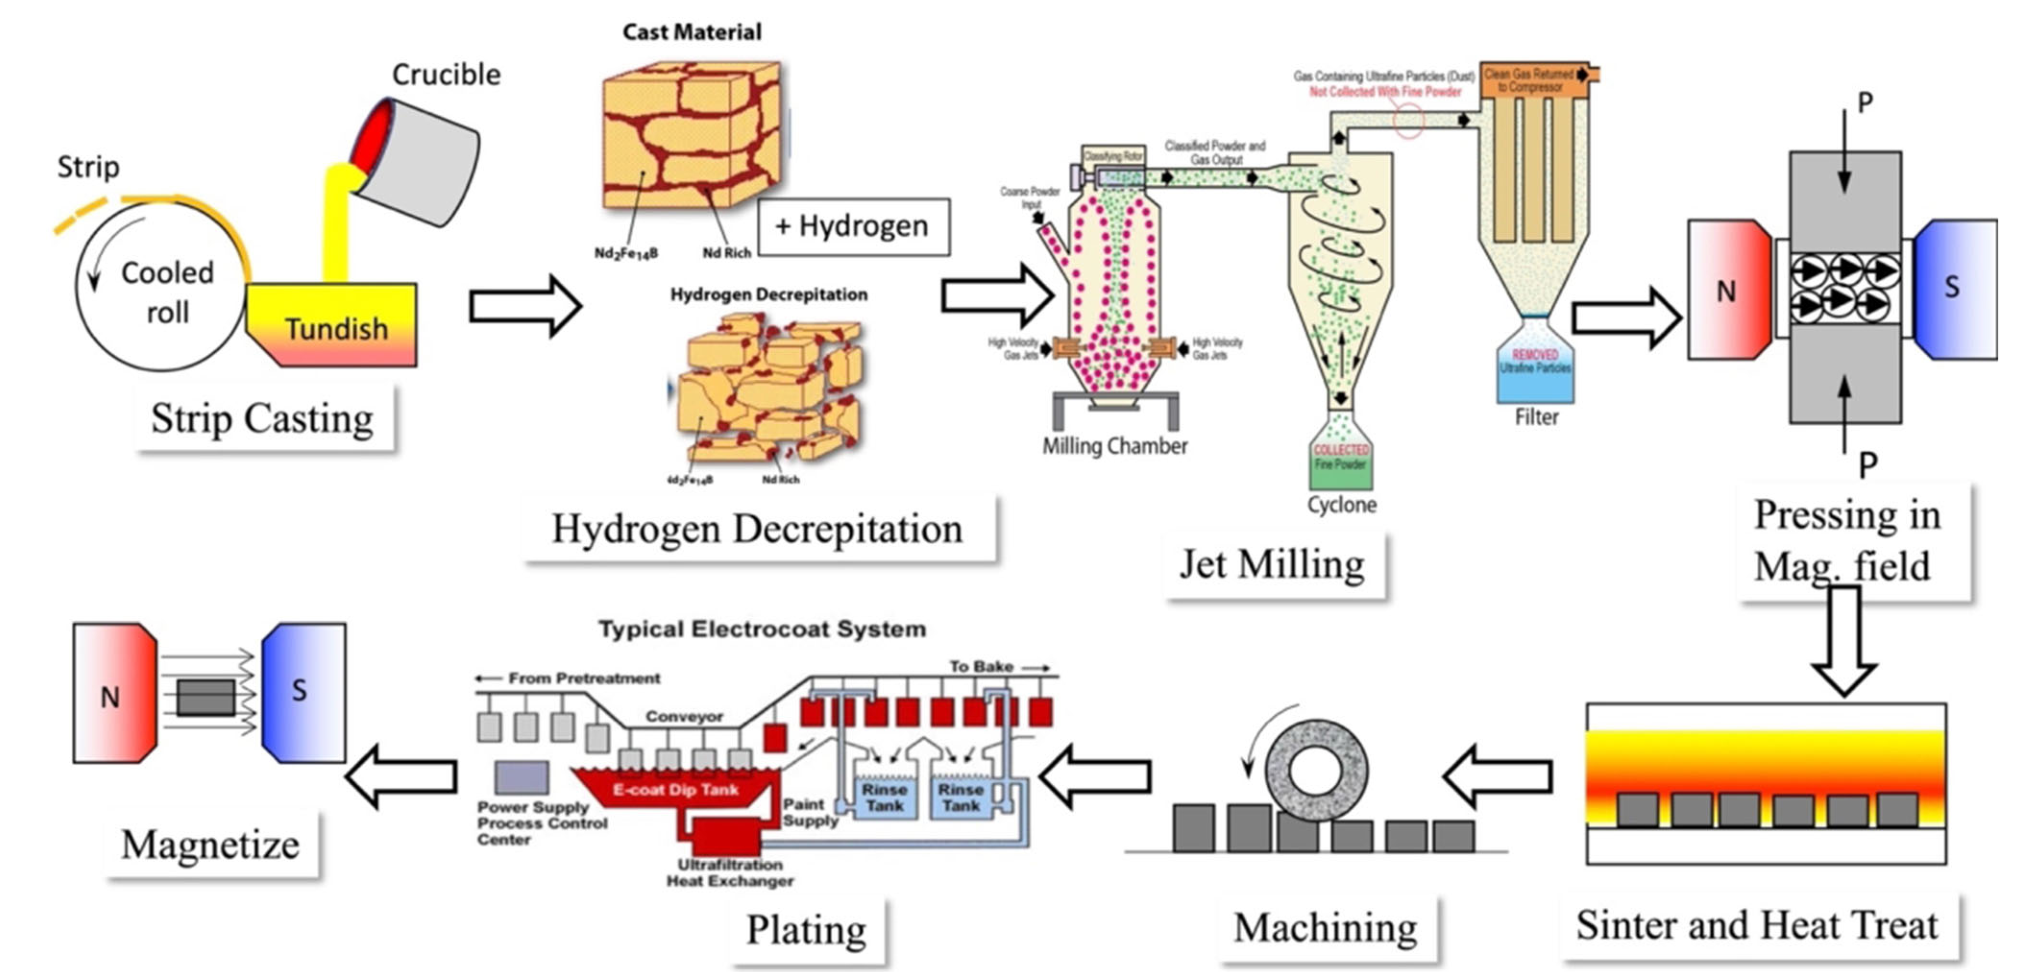
\includegraphics[height=0.65\textheight]{fig/lec02/Production_process_NdFeB_magnets.png}
            \caption{Basic process steps for the NdFeB-based magnets (source: \href{https://link.springer.com/article/10.1007/S11837-022-05156-9}{Springer JOM}, J. Cui et al., \href{https://creativecommons.org/licenses/by/4.0/}{CC BY 4.0})}
        \end{figure}
\end{frame}

%%%%%%%%%%%%%%%%%%%%%%%%%%%%%%%%%%%%%%%%%%%%%%%%%%%%%%%%%%%%%
%% Electromagnetic induction (Maxwell–-Faraday equation) %%
%%%%%%%%%%%%%%%%%%%%%%%%%%%%%%%%%%%%%%%%%%%%%%%%%%%%%%%%%%%%%
\begin{frame}
	\frametitle{Electromagnetic induction (Maxwell -- Faraday equation)}
    \begin{columns}
		\begin{column}{0.6\textwidth}
            A changing magnetic field induces an electric field according to the Maxwell -- Faraday equation:
            \begin{align}
                \mbox{Integral form:} \quad & \oint_{\partial S} \bm{E} \cdot \mathrm{d}\bm{s} = -\frac{\mathrm{d}}{\mathrm{d}t}\iint_{S}\bm{B}\cdot\mathrm{d}\bm{S},\\
                \mbox{Differential form:} \quad &\nabla \times \bm{E} = -\frac{\partial \bm{B}}{\partial t}.
                \label{eq:induction_law}
            \end{align}
            Here, $\bm{E}$ is the electric field strength and $\bm{S}$ is the surface enclosed by the loop $\partial\mathcal{S}$.
            \begin{itemize}
                \item<2-> Lentz's law: The induced electric field opposes the change in magnetic field (negative sign above).
            \end{itemize}
		\end{column}
        \hfill
		\begin{column}{0.38\textwidth}
			\begin{figure}
				\centering
				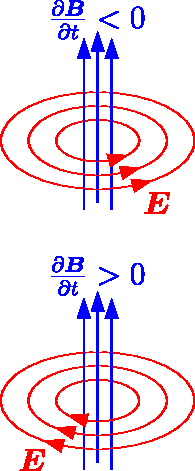
\includegraphics[height=0.6\textheight]{fig/lec02/Electromagnetic_induction.pdf}
				\caption{Representation of the magnetic and electric field relation (adapted from: \href{https://commons.wikimedia.org/wiki/File:Electromagnetic_induction.svg}{Wikimedia Commons}, Qniemiec, \href{https://creativecommons.org/licenses/by-sa/3.0/deed.en}{CC BY-SA 3.0})}
			\end{figure}
		\end{column}
		\end{columns}
\end{frame}

%%%%%%%%%%%%%%%%%%%%%%%%%%%%%%%%%%%%%%%%%%%%%%%%%%%%%%%%%%%%%
%% Electromotive force (EMF) and electromagnetic induction %%
%%%%%%%%%%%%%%%%%%%%%%%%%%%%%%%%%%%%%%%%%%%%%%%%%%%%%%%%%%%%%
\begin{frame}
	\frametitle{Electromotive force (EMF) and electromagnetic induction}
    \begin{columns}
		\begin{column}{0.55\textwidth}
            If the integration path $\partial S$ is identical to a conductor loop, the changing magnetic field induces a voltage $u_\mathrm{i}$ (electromotive force, EMF) according to Faraday's law:
            \begin{align*}
                u_\mathrm{i} =\oint_{\partial\mathcal{S}} \bm{E} \cdot \mathrm{d}\bm{s} = -\frac{\mathrm{d}}{\mathrm{d}t}\iint_{S}\bm{B}\cdot\mathrm{d}\bm{S}.
            \end{align*}
        \begin{itemize}
            \item<2-> Despite its name, the term EMF does not describe a force in the physical sense (as $u_\mathrm{i}$ is obviously a voltage).
            \item<3-> The term remains a historical artifact from the early days of electrical engineering, but is still frequently used in today's literature. 
        \end{itemize}
		\end{column}
        \hfill
		\begin{column}{0.45\textwidth}
			\begin{figure}
				\centering
				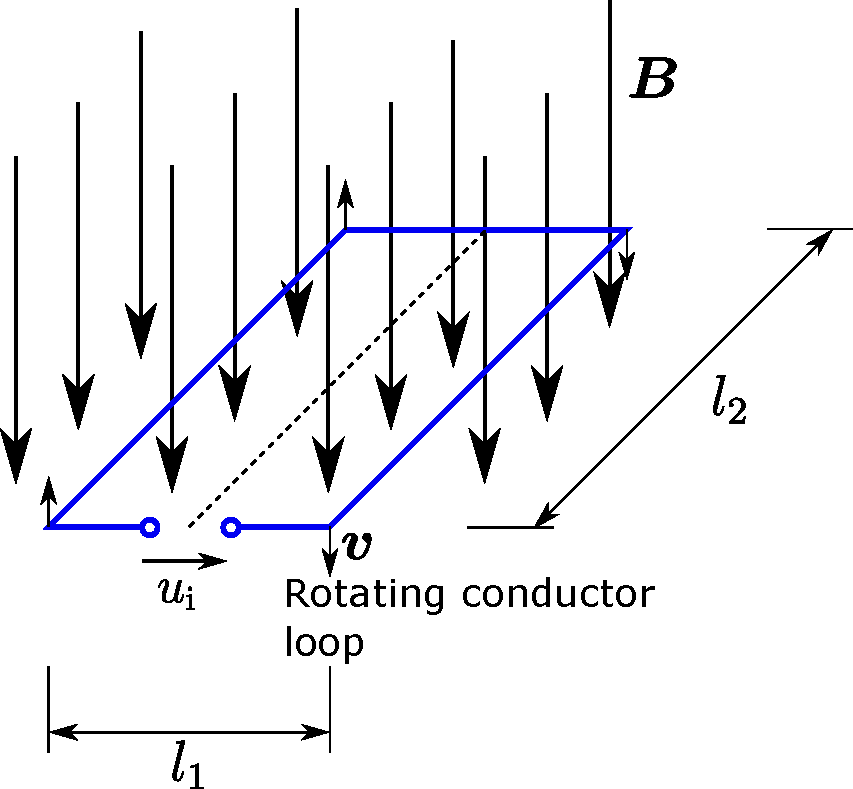
\includegraphics[height=0.6\textheight]{fig/lec02/Conductor_loop_induction.pdf}
				\caption{Induced voltage / EMF in a rotating conductor loop (adapted from: \href{https://commons.wikimedia.org/wiki/File:Leiterschleife.svg}{Wikimedia Commons}, M. Lenz, \href{https://creativecommons.org/publicdomain/zero/1.0/deed.en}{CC0 1.0})}
			\end{figure}
		\end{column}
		\end{columns}
\end{frame}

%%%%%%%%%%%%%%%%%%%%%%%%%%%%%%%%%%%%%%%%%%%%%%%%%%%%%%%%%%%%%
%% Intermediate wrap up: electromagnetic principles and magnetic materials (in inductive systems) %%
%%%%%%%%%%%%%%%%%%%%%%%%%%%%%%%%%%%%%%%%%%%%%%%%%%%%%%%%%%%%%
\begin{frame}
	\frametitle{Intermediate wrap up: electromagnetic principles and magnetic materials }
    \begin{figure}
        \centering
        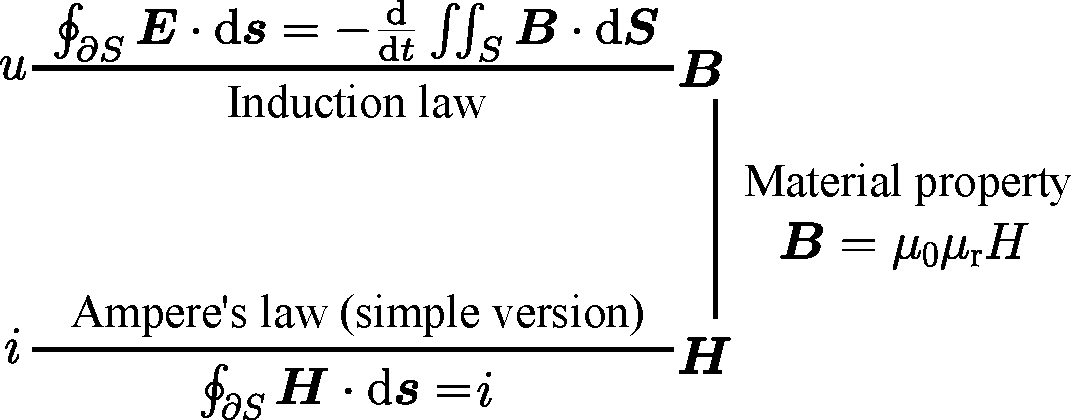
\includegraphics[height=0.5\textheight]{fig/lec02/Induction_material_ampere.pdf}
        \caption{Illustration of the connections between the phenomena discussed previously (derived from: \href{https://de.wikipedia.org/wiki/Datei:Kausalität.svg}{Wikimedia Commons}, M. Lenz, \href{https://creativecommons.org/publicdomain/zero/1.0/deed.de}{CC0 1.0})}
    \end{figure}
\end{frame}

%%%%%%%%%%%%%%%%%%%%%%%%%%%%%%%%%%%%%%%%%%%%%%%%%%%%%%%%%%%%%
%% Lorentz force %%
%%%%%%%%%%%%%%%%%%%%%%%%%%%%%%%%%%%%%%%%%%%%%%%%%%%%%%%%%%%%%
\begin{frame}
	\frametitle{Lorentz force}
    \begin{columns}
		\begin{column}{0.6\textwidth}
        The force $\bm{F}$ acting on a particle of electric charge $q$ with instantaneous velocity $\bm{v}$, due to an external electric field $\bm{E}$ and magnetic field $\bm{B}$, is given by
            \begin{equation}
                \bm{F} = q\left(\bm{E} + \bm{v}\times\bm{B}\right).
            \end{equation}
            \begin{itemize}
                \item The term $q\bm{E}$  is called the electric force.
                \item The term $q\left(\bm{v}\times\bm{B}\right)$ is called the magnetic force.
                \item In Cartesian coordinates, the Lorentz force is given by:
            \end{itemize}
            \begin{equation}
                \begin{aligned}
                    F_x &= q\left(E_x + v_yB_z - v_zB_y\right),\\
                    F_y &= q\left(E_y + v_zB_x - v_xB_z\right),\\
                    F_z &= q\left(E_z + v_xB_y - v_yB_x\right).
                \end{aligned}
            \end{equation}
		\end{column}
        \hfill
		\begin{column}{0.40\textwidth}
			\begin{figure}
				\centering
				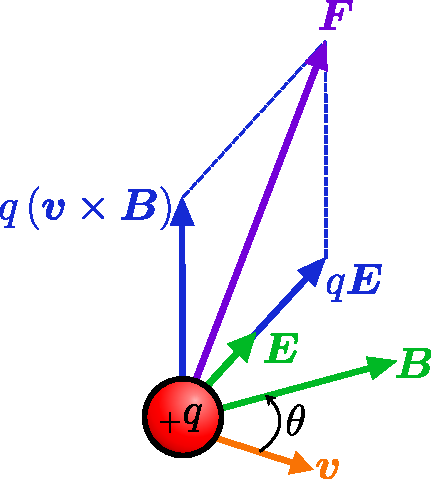
\includegraphics[height=0.5\textheight]{fig/lec02/Lorentz_force_particle.pdf}
				\caption{Lorentz force $\bm{F}$ on a particle (of charge $q$) in motion (instantaneous velocity $\bm{v}$) with given $\bm{E}$ and $\bm{B}$ fields (adapted from: \href{https://commons.wikimedia.org/wiki/File:Lorentz_force_particle.svg}{Wikimedia Commons}, Maschen, \href{https://creativecommons.org/publicdomain/zero/1.0/deed.en}{CC0})}
			\end{figure}
		\end{column}
		\end{columns}
\end{frame}

%%%%%%%%%%%%%%%%%%%%%%%%%%%%%%%%%%%%%%%%%%%%%%%%%%%%%%%%%%%%%
%% Hand rule of the magnetic Lorentz force %%
%%%%%%%%%%%%%%%%%%%%%%%%%%%%%%%%%%%%%%%%%%%%%%%%%%%%%%%%%%%%%
\begin{frame}
	\frametitle{Hand rule of the magnetic Lorentz force}
    \begin{figure}
        \centering
        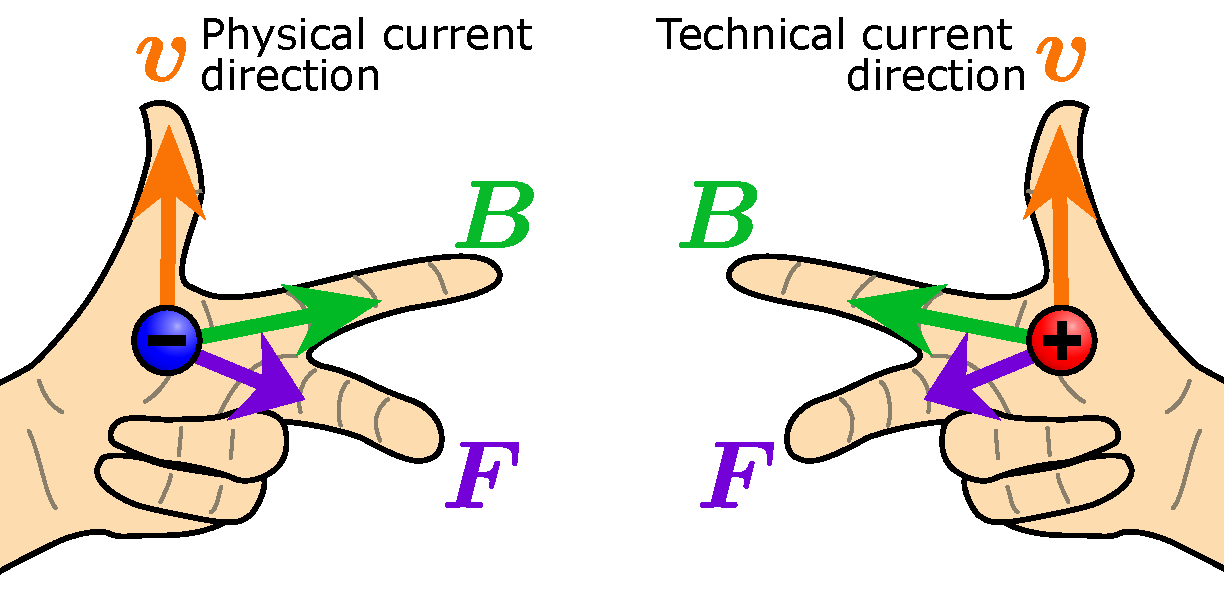
\includegraphics[height=0.6\textheight]{fig/lec02/Hand-rule-charges-both-hands.pdf}
        \caption{Right and left hand rule for the magnetic Lorentz force $q\left(\bm{v}\times\bm{B}\right)$ (adapted from: \href{https://commons.wikimedia.org/wiki/File:Right-hand-rule-charges-both-hands.svg}{Wikimedia Commons}, M. Run, \href{https://creativecommons.org/licenses/by-sa/3.0/deed.en}{CC BY-SA 3.0})}
    \end{figure}
\end{frame}

%%%%%%%%%%%%%%%%%%%%%%%%%%%%%%%%%%%%%%%%%%%%%%%%%%%%%%%%%%%%%
%% Lorentz force density for a continuous charge distribution %%
%%%%%%%%%%%%%%%%%%%%%%%%%%%%%%%%%%%%%%%%%%%%%%%%%%%%%%%%%%%%%
\begin{frame}
	\frametitle{Lorentz force density for a continuous charge distribution}
    \begin{columns}
		\begin{column}{0.5\textwidth}
         For a continuous charge distribution in motion, the Lorentz force density (force per unit volume) becomes: 
            \begin{equation}
                \bm{f} = \rho\bm{E} + \bm{J}\times\bm{B}.
            \end{equation}
            \begin{itemize}
                \item $\rho$ is the charge density (charge per unit volume).
                \item $\bm{J} = \rho \bm{v}$ is the current density.
            \end{itemize}
		\end{column}
        \hfill
		\begin{column}{0.5\textwidth}
			\begin{figure}
				\centering
				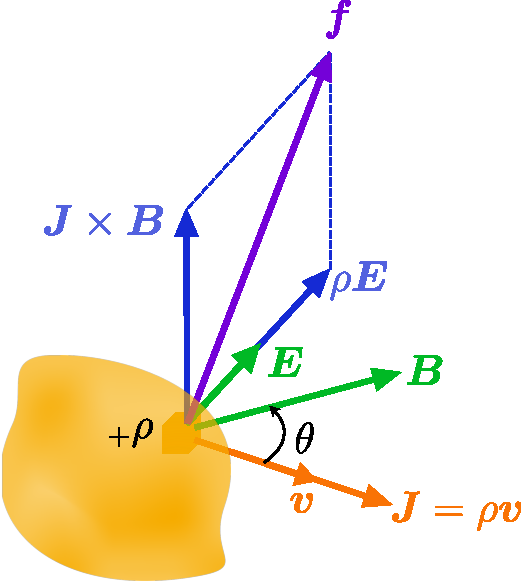
\includegraphics[height=0.6\textheight]{fig/lec02/Lorentz_force_continuum.pdf}
				\caption{Lorentz force density $\bm{f}$ on a continuous charge distribution (charge density $\rho$) in motion (adapted from: \href{https://commons.wikimedia.org/wiki/File:Lorentz_force_continuum.svg}{Wikimedia Commons}, Maschen, \href{https://creativecommons.org/publicdomain/zero/1.0/deed.en}{CC0})}
			\end{figure}
		\end{column}
		\end{columns}
\end{frame}

%%%%%%%%%%%%%%%%%%%%%%%%%%%%%%%%%%%%%%%%%%%%%%%%%%%%%%%%%%%%%
%% Magnetic networks %%
%%%%%%%%%%%%%%%%%%%%%%%%%%%%%%%%%%%%%%%%%%%%%%%%%%%%%%%%%%%%%
\begin{frame}
	\frametitle{Magnetic networks}
	\begin{columns}
		\begin{column}{0.575\textwidth}
			\begin{itemize}
                \item \textbf{Motivation}: Model magnetic systems with a simplified lumped-parameter approach and apply analysis techniques analogous to electric networks.
                \item \textbf{Assumption}: magnetic field is homogenous within a lumped element (cf. \figref{fig:Reluctance_element}).
                \item The magnetic flux per element is:
                \begin{equation}
                    \phi_k = A_k B_k .
                \end{equation}
                \item The magnetic voltage (magnetomotive force -- MMF) per element is:
                \begin{equation}
                    \theta_k = l_k H_k .
                \end{equation}
            \end{itemize}
		\end{column}
        \hfill
		\begin{column}{0.425\textwidth}
			\begin{figure}
				\centering
				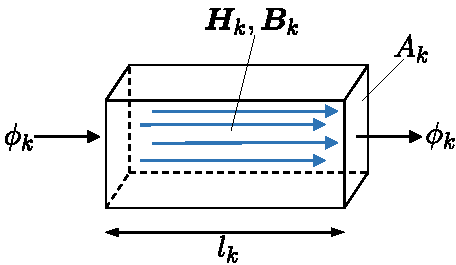
\includegraphics[height=0.4\textheight]{fig/lec02/Reluctance_element.pdf}
				\caption{Magnetic element with homogenous magnetic field}
                \label{fig:Reluctance_element}
			\end{figure}
		\end{column}
		\end{columns}
\end{frame}

%%%%%%%%%%%%%%%%%%%%%%%%%%%%%%%%%%%%%%%%%%%%%%%%%%%%%%%%%%%%%
%% Magnetic networks (cont.) %%
%%%%%%%%%%%%%%%%%%%%%%%%%%%%%%%%%%%%%%%%%%%%%%%%%%%%%%%%%%%%%
\begin{frame}
	\frametitle{Magnetic networks (cont.)}
	\begin{columns}
		\begin{column}{0.575\textwidth}
			\begin{itemize}
                \item The magnetic reluctance per element is:
                \begin{equation}
                    R_k = \frac{\theta_k}{\phi_k} = \frac{l_k}{\mu_0\mu_{\mathrm{r}k}A_k}.
                \end{equation}
                \item The magnetic conductivity (or permeance) per element is:
                \begin{equation}
                    \Lambda_k = \frac{1}{R_k} = \frac{\mu_0\mu_{\mathrm{r}k}A_k}{l_k}.
                \end{equation}
                \item As the magnetic field is free of sources ($\nabla \cdot \bm{B}=0$), it follows (node rule -- analogous to Kirchhoff's first law):
                \begin{equation}
                    \sum_k \phi_k = 0.
                \end{equation}
            \end{itemize}
		\end{column}
        \hfill
		\begin{column}{0.425\textwidth}
			\begin{figure}
				\centering
				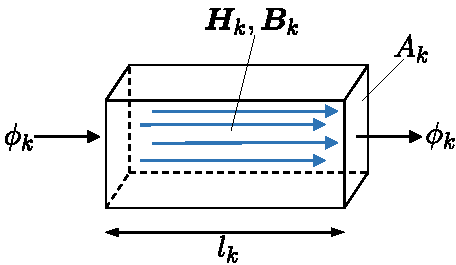
\includegraphics[height=0.4\textheight]{fig/lec02/Reluctance_element.pdf}
            \end{figure}
		\end{column}
		\end{columns}
\end{frame}

%%%%%%%%%%%%%%%%%%%%%%%%%%%%%%%%%%%%%%%%%%%%%%%%%%%%%%%%%%%%%
%% Magnetic networks (cont.) %%
%%%%%%%%%%%%%%%%%%%%%%%%%%%%%%%%%%%%%%%%%%%%%%%%%%%%%%%%%%%%%
\begin{frame}
	\frametitle{Magnetic networks (cont.)}
    Considering magnetostatic situations where the displacement current can be neglected, Amp\`ere's law reads:
    \begin{equation}
        \oint_{\partial S} \bm{H} \cdot \mathrm{d}\bm{s} = I_{\mathrm{f}} = N I = \sum_k  \theta_k = \sum_k l_k H_k.
    \end{equation}
    So far, the equation has not the structure of the second Kirchhoff’s law (loop rule). However, we can force this desired format by placing the term with the electric currents on the left-hand side of the equation:
    \begin{equation}
         \sum_k \theta_k - \theta_0 = 0 \quad \mbox{with} \quad \theta_0 = N I \,\,\mbox{(MMF term)}.
    \end{equation}
\end{frame}

%%%%%%%%%%%%%%%%%%%%%%%%%%%%%%%%%%%%%%%%%%%%%%%%%%%%%%%%%%%%%
%% Comparison: electric and magnetic network quantities %%
%%%%%%%%%%%%%%%%%%%%%%%%%%%%%%%%%%%%%%%%%%%%%%%%%%%%%%%%%%%%%
\begin{frame}
	\frametitle{Comparison: electric and magnetic network quantities}
    \begin{table}
        \centering
        \begin{tabular}{lcclcc}
            \toprule
            \textbf{Electric network} & & & \textbf{Magnetic network} & & \\
            \midrule
            Voltage & $u = \int \bm{E} \cdot \mathrm{d}\bm{s}$ & \si{\volt}&  Magnetomotive force & $\theta = \int \bm{H} \cdot \mathrm{d}\bm{s}$  & \si{\ampere}\\
            Electric field & $\bm{E}$ & \si{\volt\per\metre} & Magnetic field  & $\bm{H}$ & \si{\ampere\per\metre}\\
            Current & $i$ & \si{\ampere} & Magnetic flux & $\phi$  & \si{\volt\second}\\
            Resistance & $R$ & \si{\ohm} & Reluctance & $R$  & \si{\per\henry}\\
            Conductance & $G$ & \si{\siemens} & Permeance & $\Lambda$ &  \si{\henry}\\
            Conductivity & $\sigma$ & \si{\siemens\per\metre} & Permeability & $\mu$ &\si{\henry\per\metre}\\
            Ohm's law & $u = R i$ & & Hopkinson's law & $\theta = R \phi$ &\\
            Kirchoff'S first law & $\sum i_k = 0$ & & Kirchoff's first law & $\sum \phi_k = 0$ &\\
            Kirchoff's second law & $\sum u_k = 0$ & & Kirchoff's second law & $\sum \theta_k - \theta_0 = 0$ &\\
            \bottomrule
        \end{tabular}
        \caption{Electric and magnetic network quantities and their analogies}
        \label{eq:network_quantities}
    \end{table}
\end{frame}


%%%%%%%%%%%%%%%%%%%%%%%%%%%%%%%%%%%%%%%%%%%%%%%%%%%%%%%%%%%%%
%% Comparison: electric and magnetic network quantities %%
%%%%%%%%%%%%%%%%%%%%%%%%%%%%%%%%%%%%%%%%%%%%%%%%%%%%%%%%%%%%%
\begin{frame}
	\frametitle{Magnetic network example: simple magnetic actuator}
    \begin{figure}
		\centering
		\begin{subfigure}[b]{0.49\textwidth}
			\centering
			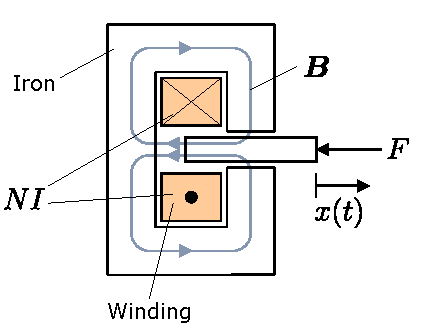
\includegraphics[width=0.7\textwidth]{fig/lec02/Magnetic_actuator_example.pdf}
            \vspace{0.4cm}
			\caption{Simple magnetic actuator}
		\end{subfigure}
		\hfill
		\begin{subfigure}[b]{0.49\textwidth}
			\centering
			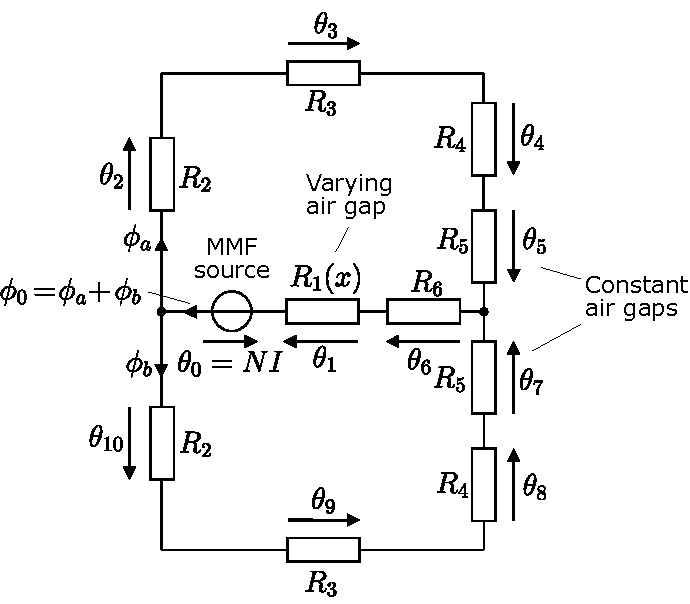
\includegraphics[width=0.8\textwidth]{fig/lec02/Magnetic_actuator_example_reluctance_network.pdf}
			\caption{Magnetic network representation of the actuator}
		\end{subfigure}
		\caption{Example for a simple magnetic actuator and its magnetic network representation} 
        \label{fig:magnetic_reluctance_network_examples}
	\end{figure}
\end{frame}

%%%%%%%%%%%%%%%%%%%%%%%%%%%%%%%%%%%%%%%%%%%%%%%%%%%%%%%%%%%%%
%% Eddy currents %%
%%%%%%%%%%%%%%%%%%%%%%%%%%%%%%%%%%%%%%%%%%%%%%%%%%%%%%%%%%%%%
\begin{frame}
	\frametitle{Eddy currents}
    \begin{columns}
		\begin{column}{0.5\textwidth}
            \begin{itemize}
                \item  A changing magnetic field induces a voltage.
                \item In bulky conductive materials (e.g., electromagnetic steel) this voltage drives currents called eddy currents.
                \item Eddy currents lead to energy losses and heat dissipation.
                \item<2-> To reduce eddy currents, laminated cores are used as they decrease the effective current path width and, therefore, increase the effective resistance per sheet.
            \end{itemize}
		\end{column}
        \hfill
		\begin{column}{0.49\textwidth}
			\begin{figure}
				\centering
				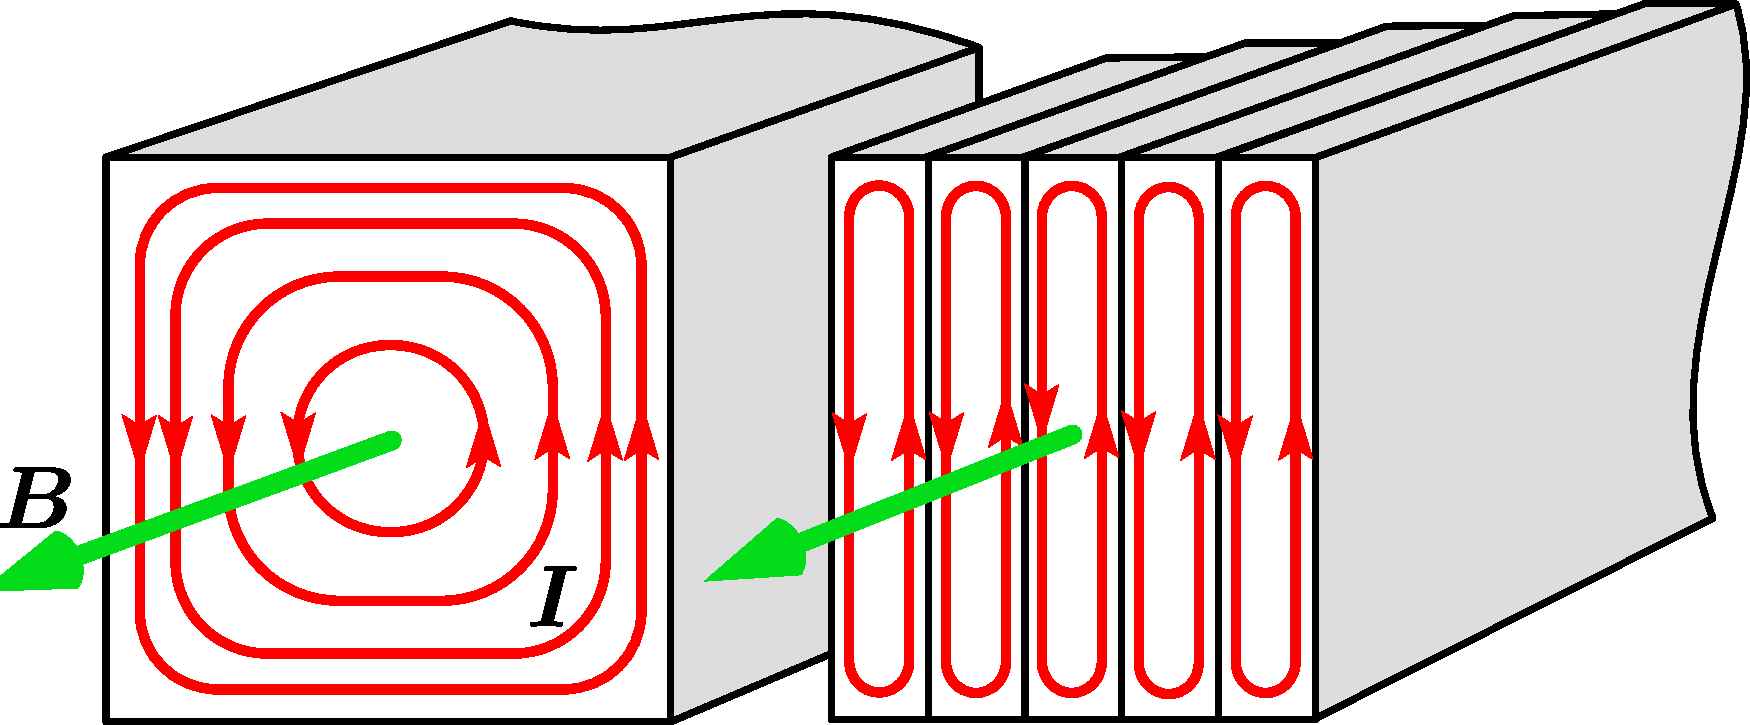
\includegraphics[height=0.36\textheight]{fig/lec02/Laminated_core_eddy_currents.pdf}
				\caption{Eddy current formations in solid and laminated steel cores (source: \href{https://commons.wikimedia.org/wiki/File:Laminated_core_eddy_currents.svg}{Wikimedia Commons}, Chetvorno, \href{https://creativecommons.org/publicdomain/zero/1.0/deed.en}{CC0})}
			\end{figure}
		\end{column}
		\end{columns}
\end{frame}

%%%%%%%%%%%%%%%%%%%%%%%%%%%%%%%%%%%%%%%%%%%%%%%%%%%%%%%%%%%%%
%% Eddy currents: single sheet example %%
%%%%%%%%%%%%%%%%%%%%%%%%%%%%%%%%%%%%%%%%%%%%%%%%%%%%%%%%%%%%%
\begin{frame}
	\frametitle{Eddy currents: single sheet example}
    \begin{columns}
		\begin{column}{0.5\textwidth}
            \begin{varblock}{Assumption}
                Sheet's thickness $d$ is much smaller than the sheet's width $w$ and the magnetic flux density $\bm{B}$ is homogenous in the normal direction of $S$ and introduces a sinusoidal excitation $\bm{B}(x,y,t) = \hat{B}\sin(\omega t)$.
             \end{varblock}
            \onslide<2->{From \eqref{eq:induction_law} integrating over $S$, we get
            $$
                2wE(x,t) = -\frac{\partial B}{\partial t}2xw
           $$
           with $2w$ being the effective contour length of $\partial S$ and  $2xw$ being the effective surface area.}
        \end{column}
        \hfill
		\begin{column}{0.49\textwidth}
			\begin{figure}
				\centering
				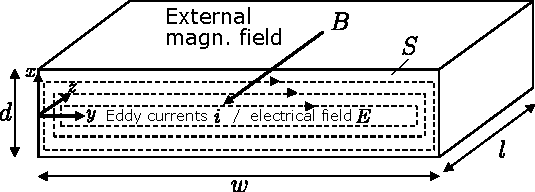
\includegraphics[height=0.3\textheight]{fig/lec02/Eddy_currents_single_sheet.pdf}
				\caption{Single sheet and induced eddy currents}
			\end{figure}
		\end{column}
		\end{columns}
\end{frame}

%%%%%%%%%%%%%%%%%%%%%%%%%%%%%%%%%%%%%%%%%%%%%%%%%%%%%%%%%%%%%
%% Eddy currents: single sheet example (cont.) %%
%%%%%%%%%%%%%%%%%%%%%%%%%%%%%%%%%%%%%%%%%%%%%%%%%%%%%%%%%%%%%
\begin{frame}
	\frametitle{Eddy currents: single sheet example (cont.)}
    With Ohm's law and the material conductivity $\sigma$, we get the current density $J$:
    $$
        J(x,t) = \sigma E(x,t) = -x\sigma\frac{\partial B}{\partial t}.
    $$\pause 
    Inserting the assumed magnetic flux density distribution it follows:
    $$
        J(x,t) = -x\sigma\omega\hat{B}\cos(\omega t).
    $$\pause
    The relative power loss (per volume) density $p(x,t)$ results in:
    $$
    p(x,t) = \frac{1}{\sigma} J^2(x,t) = x^2\sigma\omega^2\hat{B}^2\cos^2(\omega t).
    $$\pause
    The average power loss per volume (considering the $x$-direction) is:
    $$
    p(t) = \frac{1}{d} \int_{-d/2}^{d/2} p(x,t) \mathrm{d}x = \frac{1}{12}\sigma\omega^2 d^2 \hat{B}^2\cos^2(\omega t).
    $$
\end{frame}

%%%%%%%%%%%%%%%%%%%%%%%%%%%%%%%%%%%%%%%%%%%%%%%%%%%%%%%%%%%%%
%% Eddy currents: single sheet example (cont.) %%
%%%%%%%%%%%%%%%%%%%%%%%%%%%%%%%%%%%%%%%%%%%%%%%%%%%%%%%%%%%%%
\begin{frame}
	\frametitle{Eddy currents: single sheet example (cont.)}
     The average power loss per volume and time is then:
    $$
        p = \frac{1}{T}\int_0^T p(t) \mathrm{d}t = \frac{1}{24}\sigma\left(\omega d \hat{B}\right)^2.
    $$\pause
    Although this is a simplified model, it shows the significance of
    \begin{itemize}
        \item the sheet's thickness $d$,
        \item and excitation conditions $\omega$ and $\hat{B}$.
    \end{itemize}\pause
    \vspace{1em}
    This finding motivated empirical fitting approaches, like Bertotti's 
    model for the eddy currents: $$p_{\mathrm{e}}\approx k_{\mathrm{e}} f^2 \hat{B}^2 .$$
\end{frame}
